
\section{\engt{Lesson 3: LED Cube Construction} \nedt{Les 3: LED Cube constructie}}

\subsection{\engt{Layout breadboard}  \nedt{Opstelling schakelbord}}

\eng{We have all the necessary basis to start with making our Fe Cube. We start with putting all components on the breadboard. Then we test it with a program which is our previous RGB LED sketch adapted to the cube. Only when we have verified all works will we start the actual construction.

So, put following components in front of you:
\begin{enumerate}
 \item Your breadboard
 \item 9 RGB-LED (we assume common cathode in the following)
 \item 3 NPN (2N3904 normally)
 \item 9 220 $\Omega$ resistors
 \item many wires.
\end{enumerate}
First, put the RGB-LED on the board, connect the color pins with each other via wires, and connect the common cathode via a resistor to another line, see Fig.~\ref{f:lesson3_bb1}.

Connect then the resistors to pins 1 to 9. These are the pins that will feed the LED. So for a common cathode, these pins on \ardo{HIGH} will make the LED burn. Put the 3 NPN on the board. The color wire goes to the Emitter side (-) of the NPN for common cathode LED. The Colector side (+) goes to the Volt line of your breadboard. The Volt line of the breadboard goes to a 5V pin on the Arduino.

The Base leg of the NPN will control if the NPN junction is open or not. We will use pins 10, 11, 12 to control this. Your entire wiring should look like Fig.~\ref{f:lesson3_bb2}.
}

\ned{We hebben alles gezien om aan onze Fe Kubus te beginnen. We starten met alle componenten op het schakelbord te zetten. Dan testen we de schakeling met een programma die onze vorige RGB LED schets aanpast voor de kubus. Alleen als we zeker zijn dat alles werkt zullen we de effectieve constructie doen.

Plaats dus de volgende componenten voor jou:
\begin{enumerate}
 \item Jouw schakelbord
 \item 9 RGB-LED (we veronderstellen gemeenschappelijke kathode in wat volgt)
 \item 3 NPN (2N3904 normaal)
 \item 9 220 $\Omega$ weerstanden
 \item veel draden.
\end{enumerate}
Begin met de RGB-LED op je bord te zetten, verbindt de kleurpinnen met elkaar via draden, en connecteer de gemeenschappelijke kathode via een weerstand naar een andere lijn op je bord, zie Fig.~\ref{f:lesson3_bb1}.

Verbind nu de weerstanden met pinnen 1 tot 9. Deze pinnen zullen de LED van stroom voorzien. Dus, voor een gemeenschappelijke kathode zullen we deze pinnen op \ardo{HIGH} zetten om de LED te doen branden. Plaats dan de 3 NPN op het bord. De draden van een kleur gaan naar de Emitter zijde (-) van de NPN voor gemeenschappelijke kathode LEDs. De Collector zijde (+) gaat naar de Voltage lijn op je schakelbord. Deze Voltage lijn gaat dan naar een 5V pin op de Arduino.

Het Basis been van de NPN zal bepalen of de NPN junctie open is of niet. We zullen pinnen 10, 11, 12 gebruiken voor dit been. Je volledige schakeling zou er moeten uitzien als Fig.~\ref{f:lesson3_bb2}.
}

\begin{figure}
  \centering
  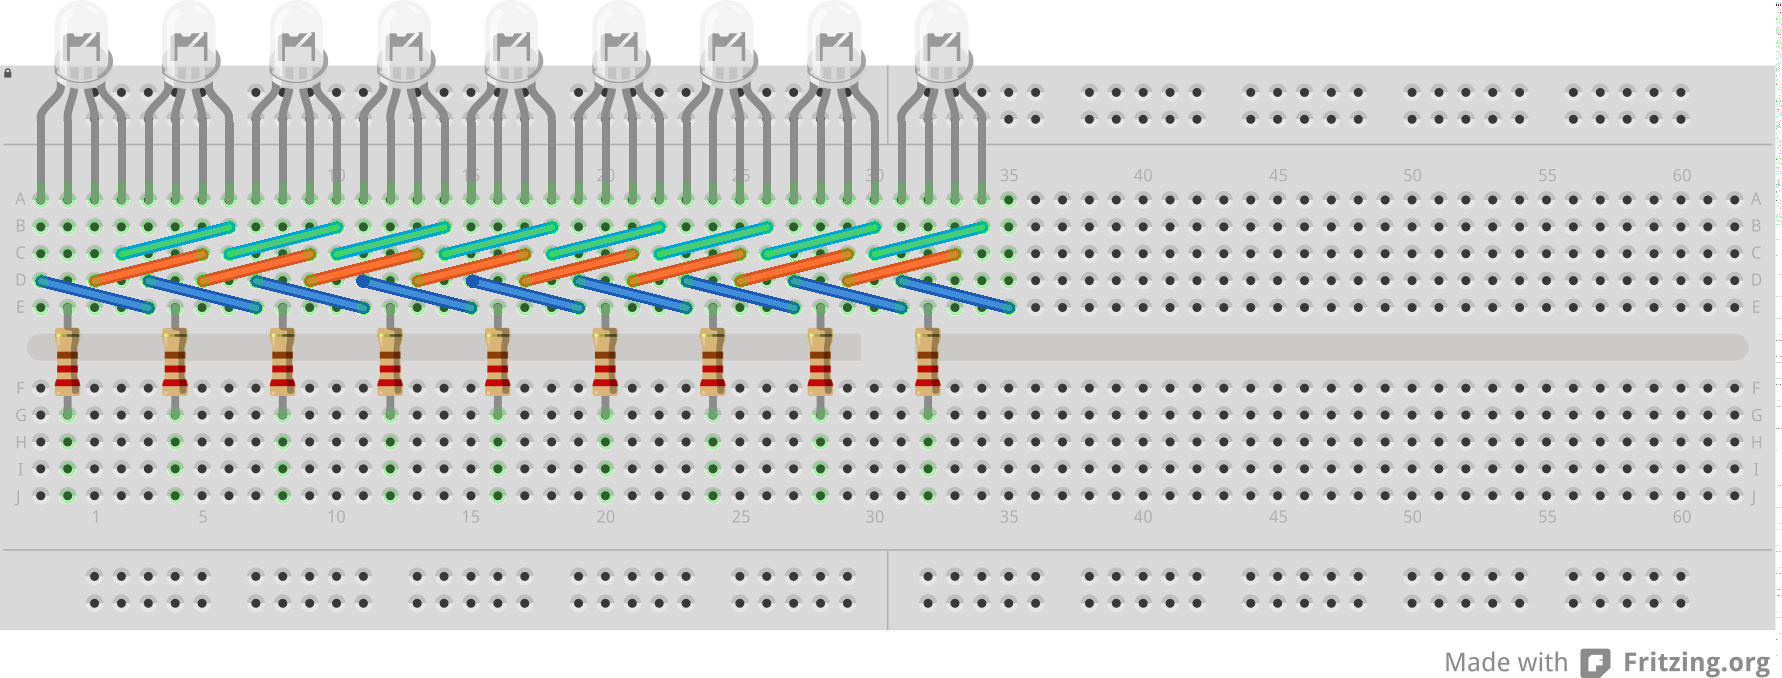
\includegraphics[width=11cm]{img/05_fecube_01_bb.png} 
\caption{\engt{Put the 9 LED on the board. Connect all equal colors to each other. The common cathode or anode goes with a 220 $\Omega$ resistor to a new line} \nedt{Plaats de 9 LED op het bord. Connecteer alle gelijke kleuren met elkaar. De gemeenschappelijke kathode of anode gaat met een 220 $\Omega$ weerstand naar een nieuwe lijn.}}
\label{f:lesson3_bb1}.
\end{figure}
%
\begin{figure}
  \centering
  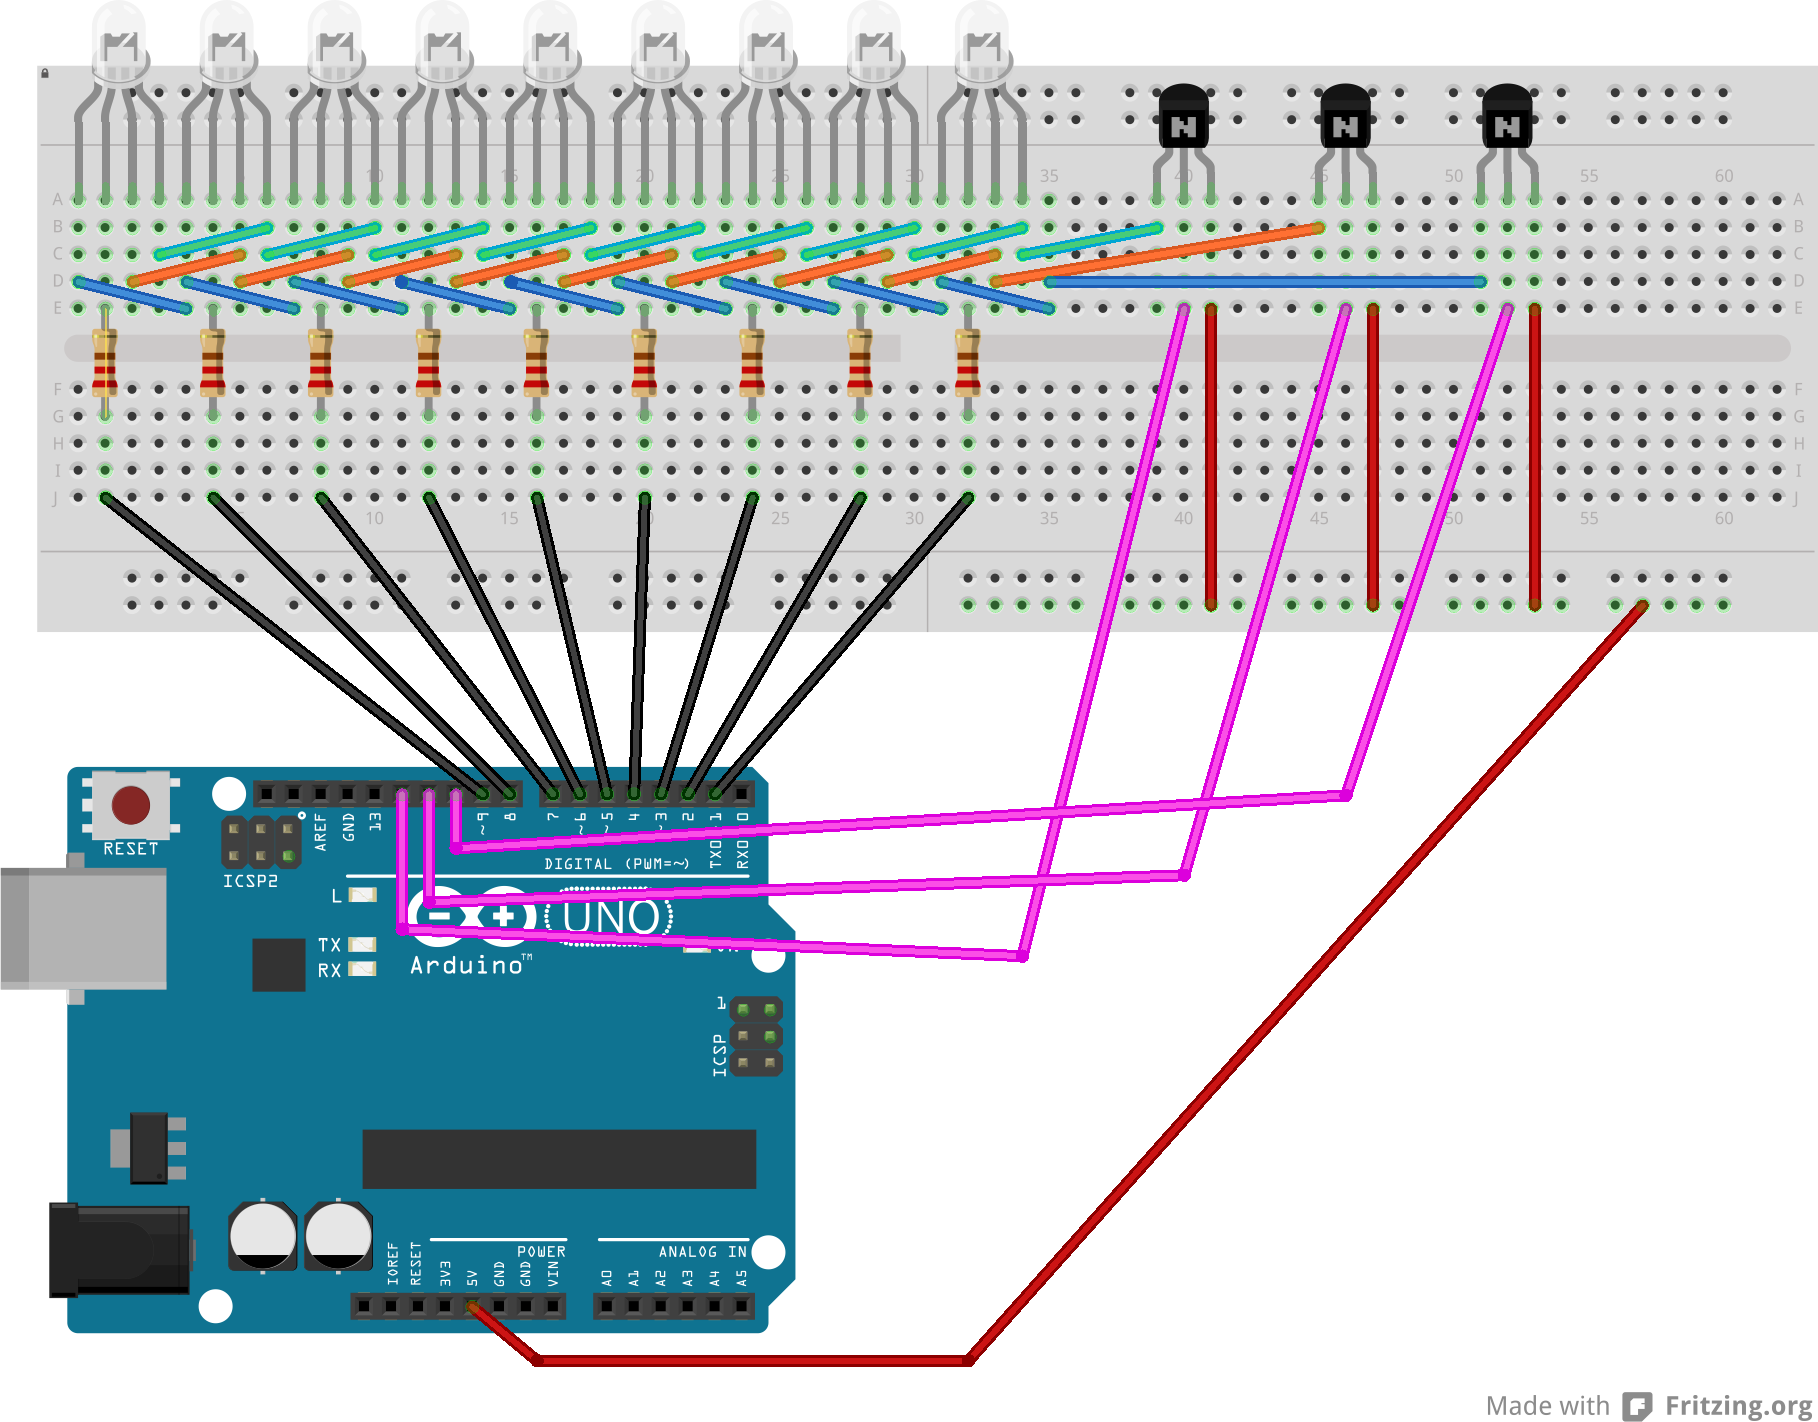
\includegraphics[width=11cm]{img/05_fecube_02_bb.png} 
\caption{\engt{Connect the resistors to pins 1 to 9. The colors go via an npn to the GND (cathode) or 5V (anode). Pins 10, 11, 12 go to the NPN to control the colors.} \nedt{Verbind de weerstanden met pinnen 1 tot 9. De kleuren gaan via een npn naar de GND (kathode) of 5V (anode). Pinnen 10, 11, 12 gaan naar de NPN om de kleuren te schakelen.}}
\label{f:lesson3_bb2}
\end{figure}

\subsection{\engt{Testing breadboard Fe Cube}  \nedt{Schakelbord Fe Cube uittesten}}

\eng{We will only verify we can make the breadboard Fe Cube work. For this we adapt our RGB sketches. We will make a movie showing  4 seconds red, then 4 seconds green, then 4 seconds blue, then 1 minute a random color, then smooth transitions for 1 minute.

This means we need all the shots we created for the RGB LED in the previous lesson, and need to create an adapted \ardo{movie} function to connect the shots as we want. We also need to change the start so that instead of only one led pin, we start up 9 led pins. 

In our previous script, we had ledR, ledG, ledB, which are easy to understand names. The LED was called led1, so we could use led1 to led9. This is not very helpfull if you want to program certain light effects. So, let's give them better names. We have a top layer (T), and a bottom (B) layer, and a single LED in the middle. Then we can divide the cube in a left (L) and right (R), and in a front (F) and an aft (A). So, let's call the LEDs:
\begin{enumerate}
\item ledTLF
\item ledTLA
\item ledTRF
\item ledTRA
\item ledBLF
\item ledBLA
\item ledBRF
\item ledBRA
\item ledMID
\end{enumerate}
Open Code \ref{c:l2_d}, and save it under a new name. The changes needed are first defining all the pins:
}

\ned{We zullen enkel controleren dat we deze schakelbord variant van de Fe kubus kunnen doen werken. Hiertoe passen we onze RGB schets aan. We zullen een film maken die eerst 4 seconden rood toont, dan 4s groen, dan 4s blauw, dan 1 minuut een willekeurige kleur, en uiteindelijk gladde overgangen voor een minuut.

Dit betekent dat we al de shots die we gemaakt hebben voor de RGB LED in de vorige lessen zullen gebruiken en aanpassen. De \ardo{movie} functie zullen we zo maken dat al deze shots elkaar opvolgen. In plaats van \'e\'en RGB led hebben we er nu 9, dus dienen we deze 9 nu samen aan of af schakelen. 

In de vorige schetsen hadden we ledR, ledG en ledB, welke gemakkelijk te verstaan zijn. De LED noemden we led1. We zouden nu led1 tot led9 kunnen gebruiken, maar dat is niet handig als we later lichteffecten maken. Laat ons ze dus betere namen geven. We hebben een top (T) en een bodem (B) laag, en een enkele LED in het midden. Dan kunnen we de kubus opdelen in een links (L) en een rechts (R), en in een frontaal (F) en een achter (A). Daarom noemen we de LEDs:\begin{enumerate}
\item ledTLF
\item ledTLA
\item ledTRF
\item ledTRA
\item ledBLF
\item ledBLA
\item ledBRF
\item ledBRA
\item ledMID
\end{enumerate}
Open Code \ref{c:l2_d}, en sla het op onder een andere naam. De eerste wijziging is alle pinnen defini\"eren:
}

\inputard{\string"../sketches/Fe_cube_03_cube_test1/Fe_cube_03_cube_test1.ino\string"}{5}{11}

\eng{Next we need to define in \ardo{setup} that these are digital output pins, so:}


\ned{Vervolgens dienen we in \ardo{setup} deze pinnen als digitale output pinnen te initializeren:}

\inputard{\string"../sketches/Fe_cube_03_cube_test1/Fe_cube_03_cube_test1.ino\string"}{15}{24}

\eng{We test the cube as a single LED, so all LED are on, or all LED are off. Hence, instead of setting only led1 on, we write a function to put all LED on, and put that in \ardo{show\_subframe\_color}}

\ned{We testen de kubus als een enkele LED, dus alle LED zijn aan, of allemaal af. Bijgevolg zullen we led1 aanzetten vervangen door een functie die alle LED aan zet, welke we plaatsen in de functie \ardo{show\_subframe\_color}
}

\inputard{\string"../sketches/Fe_cube_03_cube_test1/Fe_cube_03_cube_test1.ino\string"}{217}{221}

\eng{This new function for setting the pins \textbf{on} sends a \ardo{LOW} signal to the pins, as we are connected to the LED cathode (-)}

\ned{Deze nieuwe functie om de pinnen \textbf{aan} te zetten stuurt \ardo{LOW} signalen naar de pinnen, gezien ze verbonden zijn aan de LED kathode (-)}

\inputard{\string"../sketches/Fe_cube_03_cube_test1/Fe_cube_03_cube_test1.ino\string"}{245}{251}

\eng{Finally, we need to update the \ardo{movie} function so that it would do what we want. So this function needs to be}
\ned{Als laatste dienen we de \ardo{movie} functie aan te passen zodat het zou doen wat we willen. Deze functie dient te zijn}

\inputard{\string"../sketches/Fe_cube_03_cube_test1/Fe_cube_03_cube_test1.ino\string"}{109}{148}

\eng{
In the function \ardo{movie} you see the appearance of the \ardo{switch} structure. This is a programming structure that works like a switch based on a variable. The syntax is:
}

\ned{In de functie \ardo{movie} zie je een \ardo{switch} structuur. Dit is een programmeerstructuur die werkt als een test van een variabele. De syntax is:
}

\inputard{\string"codefrag/switch.ino\string"}{1}{10}

\eng{In this switch structure, the commands for which the var is equal to one of the labels are executed from that point onwards, up to a \ardo{break;} command. It is nicer to read than a big \ardo{if} structure to test on a variable, but otherwise works just like an if structure.
}

\ned{In deze switch structuur worden de commando's voor dewelke de variabele gelijk is aan een label uitgevoerd vanaf dat label, en dit tot op het \ardo{break;} commando. Het is mooier om te lezen in code dan een grote \ardo{if} structuur om te testen op een variabele, maar werkt anders precies als een if structuur.
}


\engo{\begin{doE}
      \textbf{One LED}. To test that a single LED does indeed not shine brighter when it is alone, change the \ardo{all\_led\_on} code so that only one LED has power.
     \end{doE}
}
\nedo{\begin{doN}
      \textbf{\'E\'en LED}. Om te testen dat een LED alleen inderdaad niet helderder brandt, wijzig de \ardo{all\_led\_on} functie zodat maar \'e\'en LED aan is.
     \end{doN}
}


\subsection{\engt{Construction}  \nedt{Constructie}}
\eng{We verified all is working, time to construct the cube. For this we will take components of our breadboard, and solder the connections in a FE Cube form.
We call our cube the Fe Cube because it is organized as the Iron (Fe) metal lattice. Solid iron has a specific structure which is depicted in the \href{http://en.wikipedia.org/wiki/Atomium}{Atomium building} in Brussels, see Figure \ref{f:atomium}. 

We call this structure a \href{http://en.wikipedia.org/wiki/Cubic_crystal_system}{Body-centered cubic crystal system}, short \textbf{bcc}.  This is a cube with an extra node in the center. 
}

\ned{De schakeling werkt, tijd om de kubus te construeren. Om dit te doen zullen we de componenten van ons schakelbord een voor een nemen en solderen in de vorm van een Fe Cubus. 

We noemen onze kubus een Fe Cubus omdat het georganizeerd is zoals het Ijzer (Fe) metaal kristalrooster. Ijzermetaal heeft een specifieke structuur welke uitgebeeld wordt in het  \href{http://nl.wikipedia.org/wiki/Atomium}{Atomium gebouw} in Brussel, zie Figuur \ref{f:atomium}.

We noemen deze structuur een \href{http://en.wikipedia.org/wiki/Cubic_crystal_system}{Lichaams-gecentreerd kubisch kristalrooster}, in het kort \textbf{bcc}. 
}

\begin{figure}
  \centering
  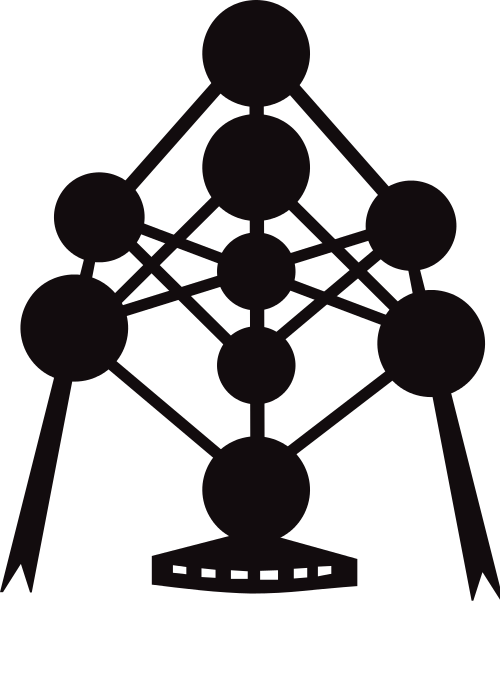
\includegraphics[width=6cm]{png/atomium.png}
\caption{\engt{Road sign depicting the Atomium building} \nedt{Wegmarkering in Brussel voor het atomium gebouw.}}
\label{f:atomium}
\end{figure}

\section{\engt{Lesson 4: Fire up the LED Cube} \nedt{Les 4: De LED Cube gebruiken}}

\subsection{\engt{Testing the Fe Cube} \nedt{De Fe Cube testen}}
\eng{You finished now constructing the cube. We need to test if all lights are working. Start with the same sketch you used for the breadboard cube. If you connect everything correctly, it should just work. 

If things are not working, you have some extra soldering to do: replace a blown out LED, make connections stronger, ... . Don't give up now. These are the last construction problems of your LED cube.}

\ned{De constructie is af. We dienen nu te teseten of alle lichten correct werken. Start met dezelfde schets die je gebruikte voor de schakelbord kubus. Als je alles correct verbindt zou het moeten werken!

Als er dingen niet werken heb je extra soldeerwerk voor de boeg: vervang een gesprongen LED, maak verbindingen sterker, ... . Nu niet opgeven! Dit zijn de laatste constructieproblemen voor je LED kubus.}

\subsection{\engt{Generic patterns ... and a snake} \nedt{Algemene patronen ... en een slang}}

\eng{
We have a working cube now, but we can only show single colors with our current code. Let's change that. We want to be able to write some light effects, and show that on our cube. So let us create a \ardo{movie} function that can load patterns we create. Like that we can write down a pattern, and pass it to this function. The first pattern we want to make is the snake pattern: a single light that jumps from LED to LED in the three base colors.

We need to define the data structure of a pattern. What needs to be in a pattern?
\begin{enumerate}
 \item We need for 9 LED what color they must have. A color is a RGB value like (13,50,2), assuming we still use values between 0 and 64. That is, we need $3\times 9 = 27$ numbers to form a frame now.
 \item We need to know how long to hold a frame before moving to the next frame. So, we need an extra number for the milliseconds, for a total of 28 numbers.
\end{enumerate}
Therefore, a pattern will look like a list of numbers which indicate the different frames and how long they take. For a single frame this will be:\newline
$\{$R1,G1,B1, R2,G2,B2, R3,G3,B3, R4,G4,B4, R5,G5,B5, R6,G6,B6, R7,G7,B7, R8,G8,B8, R9,G9,B9, duration$\}$\newline

The order of the LEDS in the frame will be ledTLF, ledTLA, ledTRF, ledTRA, ledBLF, ledBLA, ledBRF, ledBRA, ledMID. If a shot consists of pattern with 20 fixed frames, we create a single large array with all the frames, one after the other. As Arduino code is not that clever, we need to know somehow what the last pattern is. We could count and pass this number of patterns, but that will quickly lead to an error. Easier is to finish the list with a fake pattern with duration 0. If we read this 0, we know the pattern is finished. 

In our code, our \ardo{movie} function will use a \ardo{moviepattern} function that will handle a pattern you give it. The function will divide the pattern in shots: one shot per fixed frame. The shot will take as long as the duration you have passed in the pattern. This shot is the analogue of the \ardo{fixed\_color} for the single RGB LED: \ardo{fixed\_pattern}, which is a shot that produces a single fixed image on the cube.

There is an extra complication though. The Arduino does not have a lot of memory to work with. There is the SRAM memory with which the Arduino works, and there is Flash memory where your program will be stored. All general variables in your code need to be available at all times, so they need to be stored in SRAM memory. Our patterns can be large though, and the memory would fill up, causing the Arduino to just not produce anything anymore. To avoid this, we will store the patterns in flash memory, and only obtain the frame of the pattern we need. Because of this, you will find in the code:}
\ned{We hebben een werkende LED kubus, maar we kunnen enkel maar vaste kleuren tonen met de huidige code. Laten we dat veranderen. We willen lichteffecten kunnen programmeren. Laat ons dus een \ardo{movie} functie maken die patronen kan laden. Op deze manier kunnen we een lichtpatroon opschrijven en dat door deze functie laten laden op de kubus. Het eerste patroon die we willen maken is een slangenparoon: een enkel lichtje dat springt van LED naar LED in de 3 basiskleuren.

We moeten een data structuur maken voor het patroon. Waaruit moet een patroon bestaan?
\begin{enumerate}
 \item We dienen voor de 9 LED te weten welke kleur ze moeten hebben. Een kleur is een RGB waarde zoals  (13,50,2), ervanuit gaande dat we nog steeds waarden tussen 0 en 64 gebruiken. We hebben nu dus $3\times 9 = 27$ nummers nodig om een frame van een shot te maken.
 \item We moeten dan ook nog weten hoe lang we een enkel frame moeten aanhouden vooraleer naar het volgende frame in het patroon te schakelen. We hebben dus nog een extra nummer nodig voor het aantal milliseconden dat een frame moet getoond worden, voo een totaal van 28 nummers.
\end{enumerate}
Een patroon zal dus lijken op een lijst van nummers welke aanduiden welk frame te tonen en voor hoe lang. Voor een enkele frame zal dit zijn:\newline
$\{$R1,G1,B1, R2,G2,B2, R3,G3,B3, R4,G4,B4, R5,G5,B5, R6,G6,B6, R7,G7,B7, R8,G8,B8, R9,G9,B9, duurtijd$\}$\newline

De orde van de LEDs in het frame zal ledTLF, ledTLA, ledTRF, ledTRA, ledBLF, ledBLA, ledBRF, ledBRA, ledMID zijn. Als een shot bestaat uit een patroon met 20 vaste frames, dan zullen we een enkele grote lijst maken met alle frames, de ene na de andere. Gezien Arduino code niet zo slim is moeten we op een of andere manier doorgeven welke het laatste frame is. We zouden dit zelf kunnen tellen en doorgeven, maar dat leidt vlug tot fouten. Gemakkelijker is om te eindigen met een vals patroon met duurtijd 0. Als we deze 0 lezen weten we dat het patroon gedaan is.

In onze code zal de  \ardo{movie} functie nu een \ardo{moviepattern} functie oproepen. Deze zal het patroon afspelen die je doorgeeft. De functie zal het patroon intern verdelen in een shot per gegeven frame. Dit shot zal dan zo lang duren als de duurtijd die je opgegeven hebt in het patroon. Dit shot is de tegenhanger van de functie \ardo{fixed\_color} bij de enkele RGB LED: \ardo{fixed\_pattern}, welke een shot is dat een enkel vast beeld op de kubus toont.

Er is evenwel nog een complicatie. De Arduino heeft niet veel geheugen om mee te werken. Er is SRAM geheugen welke de Arduino mee werkt, en Flash geheugen waar het programma opgeslagen wordt. Alle globale variabelen moeten altijd beschikbaar zijn en bevinden zich dus in SRAM. Onze patronen kunnen evenwel groot zijn, en het geheugen zal dat vol geraken, waarna de Arduino stopt met werken. Om dit te vermijden zullen we de patronen opslaan in flash geheugen, en enkel het frame dat we nodig hebben laden in SRAM geheugen. Daarom zul je het volgende terugvinden in de code:
}

\inputard{\string"codefrag/defavr.ino\string"}{1}{3}

\eng{
This will define the functions we need to move data from flash memory to SRAM.
The \ardo{PROGMEM} part replaces a normal \ardo{array} construction and defines an array of integers. It indicates we want an array of integers, but we want it in \ardo{PROGMEM}, so in the memory that stores our program, the flash memory.

You call in the \ardo{movie} function the new \ardo{moviepattern} function if you want to send a pattern to the LED cube. We cannot pass a variable with the moviepattern we want to use because this is now in \ardo{PROGMEM}. You will need to edit \ardo{moviepattern} to load the correct pattern.

In the function \ardo{moviepattern} you see twice the appearance of the \ardo{switch} structure. 

In the first switch structure you need to add the start conditions of the patterns you want to show. In the second switch structure you need to copy the pattern you want into the \ardo{shotpattern} variable, as well set the \ardo{nextduration} variable to the duration of the \textit{next} shot. The function \ardo{pgm_read_word_near} is the function that will copy from the program memory (flash) to SRAM. The only thing needed to change there is the name of the pattern, or add a case with your pattern.

The start conditions for a pattern are:
\begin{enumerate}
 \item \textbf{patternscale\_start}: with what time scaling to start? This is multiplied with the duration of a frame.
 \item \textbf{patternscale\_speedup}: a value larger than 0 and less than 1. Every time the pattern is finished, you can make it go faster. This speedup is multiplied with the duration of the frames
 \item \textbf{patternscale\_min}: it has no use to go always faster, you need to stop some time. This indicates the minimum scale, after which we assume the pattern can be completely stopped.
 \item \textbf{patternrepeatmin}: as the fastest presentation at patternscale\_min will be so fast you can hardly see it, you can set with this variable how many times to repeat this fastest pattern before we really consider the pattern as finished. When the pattern is finished in this way, the label of the switch command, NRPATTERN in the sketch, is increased by one, causing a next pattern to be loaded if that is present.
 \item \textbf{totalpatterns}: we use the switch command to select the pattern. Give with this variable how many patterns in total you use. 
\end{enumerate}
To show the influence of changing these parameters, the code has an extra pattern called PatternCircle, which uses different starting values.

The rest of the extra code is to compute the correct speedup of the shots in the pattern, and to determine correctly when a pattern is finished and the next pattern can begin.
}

\ned{Dit definieert de functies die we nodig hebben om data te verplaatsen van flash naar SRAM.  Het  \ardo{PROGMEM} gedeelte vervangt een gewone lijst (\ardo{array}) constructie en maakt voor ons een lijst van integers (gehele getallen, ons patroon dus). Het duidt aan dat we een lijst integers willen, maar dat we die in \ardo{PROGMEM} willen, dus in flash.

In de functie \ardo{moviepattern} zie je twee keer een \ardo{switch} structuur. 

In de eerste switch structuur dien je de startcondities van je patroon te schrijven. In de tweede switch structuur dien je je patroon te copi\"eren in de \ardo{shotpattern} variabele, alsook de \ardo{nextduration} variabele opvullen met de duur van het \textit{volgende} shot. De functie \ardo{pgm_read_word_near}  is de functie die zal copi\"eren van programma geheugen (flash) naar SRAM. Het enige dat je hier normaal moet wijzigen is de naam van je patroon, of het toevoegen van een switch case voor jouw patroon.

De startcondities van een patroon zijn:
\begin{enumerate}
 \item \textbf{patternscale\_start}: met welke tijdsschaling wil je beginnen. deze schaal wordt vermenigvuldigd met de duur van een frame.
 \item \textbf{patternscale\_speedup}: een waarde tussen 0 en 1. Elke keer een patroon gedaan is kun je het hiermee vlugger doen gaan. Deze speeup wordt ook vermenigvuldigd met de duur van een frame.
 \item \textbf{patternscale\_min}: je kan niet altijd maar sneller gaan, je moet ook eens stoppen. Deze parameter bepaald de minimum tijdsschaling, na dewelke het patroon volledig kan stoppen.
 \item \textbf{patternrepeatmin}: gezien de snelste weergave met patternscale\_min vaak zo vlug gaat dat je het niet kunt zien, kun je hier opgeven hoe vaak deze snelste weergave moet herhaald worden. Daarna zullen we het patroon defenitief als gedaan beschouwen, en wordt NRPATTERN met 1 verhoogd. NRPATTERN is de variabele die in de switch structuren gebruikt wordt. Het verhogen met een zal dus zorgen dat een volgend patroon uitgevoerd wordt.
 \item \textbf{totalpatterns}: gebruik deze variabele om aan te duiden hoeveel patronen er in totaal zijn. 
\end{enumerate}
Om te tonen wat de invloed van deze parameters is bevat de code een extra patroon: PatternCircle. Deze heeft andere startwaarden en gedraagd zich dus anders.

De rest van de extra code is dan om de correcte versnelling van de shots in een patroon te berekenen, en om te bepalen of een patroon gedaan is en een nieuwe kan beginnen.
}

\eng{
The entire code is given in Code \url{https://github.com/ingegno/fecube/blob/master/sketches/Fe_cube_03_cube_pattern/Fe_cube_03_cube_pattern.ino} %\ref{c:ledcube_snake}.
}

\ned{
De vollige code kun je vinden op \url{https://github.com/ingegno/fecube/blob/master/sketches/Fe_cube_03_cube_pattern/Fe_cube_03_cube_pattern.ino} %\ref{c:ledcube_snake}.
}

% \begin{code}\label{c:ledcube_snake}
%  \ \newline
% \inputardfull{\string"../sketches/Fe_cube_03_cube_pattern/Fe_cube_03_cube_pattern.ino\string"}
% \end{code}


\engo{\begin{doE}
      \textbf{Your pattern}. Time to make your own pattern. How about a rotating emergency vehicle light? Or christmass twinkle? Or ....
     \end{doE}
}
\nedo{\begin{doN}
      \textbf{Jouw patroon}. Tijd om je eigen patroon te maken. Wat denk je van een zwaailicht? Of kerstboom flikkering? Of ...
     \end{doN}
}

\subsection{\engt{Intelligent patterns ... and a beating heart} \nedt{Intelligente patronen ... en een kloppend hart}}

\eng{We can do patterns, which is nice, but patterns are a lot of work to create. This is no different in animation movies or with special effects. They take a lot of time to make. So, people use programming instead to do as much of the work as possible. 

For example, if you look at our snake pattern, we essentially repeat 3 times the same pattern but for a different color. It would be easier to write the pattern once, and then in the code shift the pattern one color. As another example, consider writing a pattern for a beating heart. We would go from no light, to always more red. When all if fully red, we would invert it. In essence, we would need to repeat the pattern in reverse order. Again, with software this would be easier and avoid us writing a long pattern. 

Before writing more software, it is important to design it somewhat. We now end a pattern with a dummy line which has duration 0. As a duration smaller than zero makes no sense, we can use a negative duration to indicate performing a specific operation on the pattern, for example reverse it as in the beating heart, or shift the colors as in the snake. Apart from this, we would need a counter also to indicate how often to extend the pattern once the end is reached. 

We will use following definitions: the variable \ardo{extend\_pattern} will contain how often the pattern must be extended when the end is reached. The final duration will indicate how the pattern must be repeated. We will consider as durations
\begin{itemize}
 \item[0]: the pattern does not change.
 \item[-1]: reverse the pattern in the next repeat
 \item[-11]: shift the colors one to the right: R$\rightarrow$G, G$\rightarrow$B, B$\rightarrow$R
 \item[-12]: shift the colors two to the right: R$\rightarrow$B, G$\rightarrow$R, B$\rightarrow$G
 \item[-90]: rotate the shot over -90 degrees. Ideal to create rotating animations.
 \item[-180]: flip the shot, so TLF becomes TRA
 \item[-270]: rotate the shot over 90 degrees
\end{itemize}

Doing all these changes will increase the amount of code. As our patterns are smaller however, we will be able to do more with less memory.
}

\ned{We kunnen nu patronen maken, maar dat is wel veel werk. Dit is niet verschillend van animatiefilms met speciale effecten. Veel tijd is nodig om die te maken. Om dit te versnellen zullen ontwikkelaars zoveel mogelijk programmeren, om zo manueel werk te besparen.

Bevoorbeeld, als we ons slangenparoon bekijken zien we in essentie hetzelfde patroon 3 keer herhaald, maar wel voor een andere kleur. Het zou makkelijker zijn het patroon \'e\'en keer schrijven, en dan met een programma het op een andere kleur toe te passen. Als een ander voorbeeld, stel dat je een kloppend hart patroon wil maken. Dan ga je van geen licht naar alle LED die rood worden. Zodra alles rood gaan we opnieuw naar geen licht, we moeten dus het patroon omdraaien. Als we dit omdraaien gewoon kunnen programmeren dan kunnen we vermijden een lang patroon te schrijven!

Vooraleer nieuwe code te schrijven is het belangrijk eerst over het ontwerp na te denken. We eindigen nu een patroon met een valse lijn met duur 0. Gezien een duur kleiner dan 0 geen zin heeft, kunnen we een negatieve duur gebruiken om een effect aan te duiden om het patroon voort te zetten. Bevoorbeeld, het patroon herhalen met een andere kleur. We zullen dan wel moeten bijhouden hoeveel keer we het patroon moeten uitbreiden met een effect, zodat we zouden weten wanneer het echte einde bereikt is. 

Laat ons volgende defenities invoeren: met de variabele \ardo{extend\_pattern} duiden we aan hoeveel keer we het patroon uitbreiden. De duurtijd van de valse eindlijn zal aanduiden hoe het patroon moet herhaald worden. We beschouwen als mogelijke duurtijden
\begin{itemize}
 \item[0]: Het patroon wijzigt niet.
 \item[-1]: keer het patroon om voor de volgende herhaling (dus van achter naar voor het patroon lezen)
 \item[-11]: wijzig de basiskleuren naar rechts, dus: R$\rightarrow$G, G$\rightarrow$B, B$\rightarrow$R
 \item[-12]: wijzig de basiskleuren naar links, dus : R$\rightarrow$B, G$\rightarrow$R, B$\rightarrow$G
 \item[-90]: roteer het shot over -90 degrees. Ideaal om roterende animaties te maken.
 \item[-180]: flip het shot, dus TLF wordt TRA
 \item[-270]: roteer het shot over 90 graden
\end{itemize}

Al deze wijzigingen zullen de hoeveelheid code doen toenemen. Onze patronen kunnen evenwel kleiner zijn, waardoor we minder geheugen moeten gebruiken.

}

\eng{So, the patterns can be shorter. Here are the two patterns we consider, our snake of before, and the beating heart.}

\ned{De patronen kunnen dus korter zijn. Hier zijn de twee patronen die we beschouwen, onze slang van eerder, en een kloppend hart.}

\inputard{\string"../sketches/Fe_cube_03_cube_intpattern/Fe_cube_03_cube_intpattern.ino\string"}{18}{67}

%\begin{code}\label{c:ledcube_heart}
% \ \newline
%\inputardfull{\string"../sketches/Fe_cube_03_cube_intpattern/Fe_cube_03_cube_intpattern.ino\string"}
%\end{code}

\eng{All the other changes are in our \ardo{moviepattern} function. We have two extra control variables: \ardo{extend\_pattern} indicating how many times a single pattern is extended by a copy with some effects on. So, for the original snake, we reduced the 3 loops to one loop in red, so we need to extend it twice to obtain the original length.

The other new variable is \ardo{starteffect}. That is, we need not wait for an extend to apply an effect, we can do it from the start. To show what is possible with effects, we manipulate the red snake pattern in 4 different ways, as well as adding a beating heart pattern. The full code is in \url{https://github.com/ingegno/fecube/blob/master/sketches/Fe_cube_03_cube_intpattern/Fe_cube_03_cube_intpattern.ino}. Only the start of the \ardo{moviepattern} function with the two switch statements is something you would want to change for your own patterns. See Code
\ref{c:int_pat} for this start.
}

\ned{Al de andere veranderingen zijn in onze \ardo{moviepattern} functie. We hebben twee nieuwe controle variabelen: \ardo{extend\_pattern} duidt aan hoe vaak we het patroon uitbreiden met een copie met effecten toegepast. Dus, voor de originele slang reduceren we de 3 gekleurde slangen door een enkele rode, en breiden we het twee keer uit.

De andere nieuwe variabele is \ardo{starteffect}. Dit is het effect die we vanaf de start toepassen. Om te tonen wat mogelijk is met de effecten manipuleren we de rode slang op 4 verschillende manier, en voegen we het kloppend hart shot toe. De volledige code is in \url{https://github.com/ingegno/fecube/blob/master/sketches/Fe_cube_03_cube_intpattern/Fe_cube_03_cube_intpattern.ino}.
Enkel de start van de \ardo{moviepattern} functie met de twee \ardo{switch} structuren zou je moeten wijzigen om je eigen patronen te gebruiken. Zie Code \ref{c:int_pat} voor deze start.
}


\begin{code}\label{c:int_pat}
 \ \newline
\inputard{\string"../sketches/Fe_cube_03_cube_intpattern/Fe_cube_03_cube_intpattern.ino\string"}{211}{293}
\end{code}


\engo{\begin{doE}
      \textbf{More patterns}. The effects are working? Add another effect, eg a color change. Or just write a new pattern using some of the effects.
     \end{doE}
}
\nedo{\begin{doN}
      \textbf{Meer patronen}. De effecten werken op je Fe Kubus? Voeg een nieuw effect toe, bevoorbeeld een kleurverandering. Of schrijf gewoon een nieuw patroon dat van enkele effecten gebruik maakt.
     \end{doN}
}

\newpage
\section{\engt{Lesson 5: Interaction with a push button} \nedt{Les 5: Interactie met een drukknop}}

\eng{You can do wonderful things with your cube. But it would be nice if it was a bit more user friendly. Would it not be super if we could interact with the cube? For example, change effect when we push a button? Or change your cube into a dice that you roll when you push on a button.
}
\ned{Je kan prachtige dingen doen met je kubus. Maar we kunnen het nog wat gebruiksvriendelijker maken. Ware het niet super als je kon interageren met je kubus? Bevoorbeeld van effect veranderen als je een knop drukt? Of je kubus omtoveren in een dobbelsteen die je rolt als je op de knop drukt...}

\subsection{\engt{How does a push button work?} \nedt{Hoe werkt een drukknop?}}

\eng{Take the push button. You see 4 pins, and a button you can push down, but which jumps back to the start position when you release it. There are two pins on one side, and two on the opposite side. Put the button with one side with pins towards you, and one away. 
Normally the pins on the left are connected, and the pins on the right also. Then, when you press the button, the left and the right will be connected.

Why 4 pins and not 2? Well, this makes it easier to solder. Normally you will need to connect more than two wires to the button, and having a different pin to solder to is easier. 

To verify you understand what pin is what, we make a little circuit with a LED, a 330$\Omega$ resistor, and the push button. Use the push button to interrupt the power to the LED, and use your 5V and GND pins on the Arduino to provide current. No code is needed, you could also use a 3V coin button battery for this exercise.

The wiring is given in Figure \ref{f:lesson5_pbtn1}. If you push the button the light should switch on.
}

\ned{Neem een drukknop. Je ziet 4 pinnen en een knop die je kan indrukken, maar welke terugkeert naar de beginpositie zodra je loslaat. Er zijn twee pinnen aan een zijde, en twee aan de overstaande zijde. Leg de knop zo dat een zijde met pinnen naar je toe, en de andere van je weg. Normaal gezien zijn de pinnen links verbonden met elkaar, alsook die rechts. Als je de knop indrukt worden ook links en rechts met elkaar verbonden.

Waarom 4 pinnen en niet 2? Dit is omdat het makkelijker solderen is zo. Je zal vaak meer dan 2 draden aan een knop moeten bevestigen, en dus zijn twee extra pinnen handig.

Om te zien of je goed begrijpt welke pin wat doet maken we een klein circuit met een LED, een 330$\Omega$ weerstand en een drukknop. Gebruik de drukknop om de stroom naar de LED te onderbreken, en gebruik de 5V en GND pinnen van de Arduino om stroom te leveren. Je hebt geen code nodig, en je zou ook een 3V knoopbatterij kunnen gebruiken voor deze oefening.

Het schema is gegeven in Figuur \ref{f:lesson5_pbtn1}. Als je de knop indrukt zou het licht aan moeten gaan.
}
\begin{figure}
  \centering
  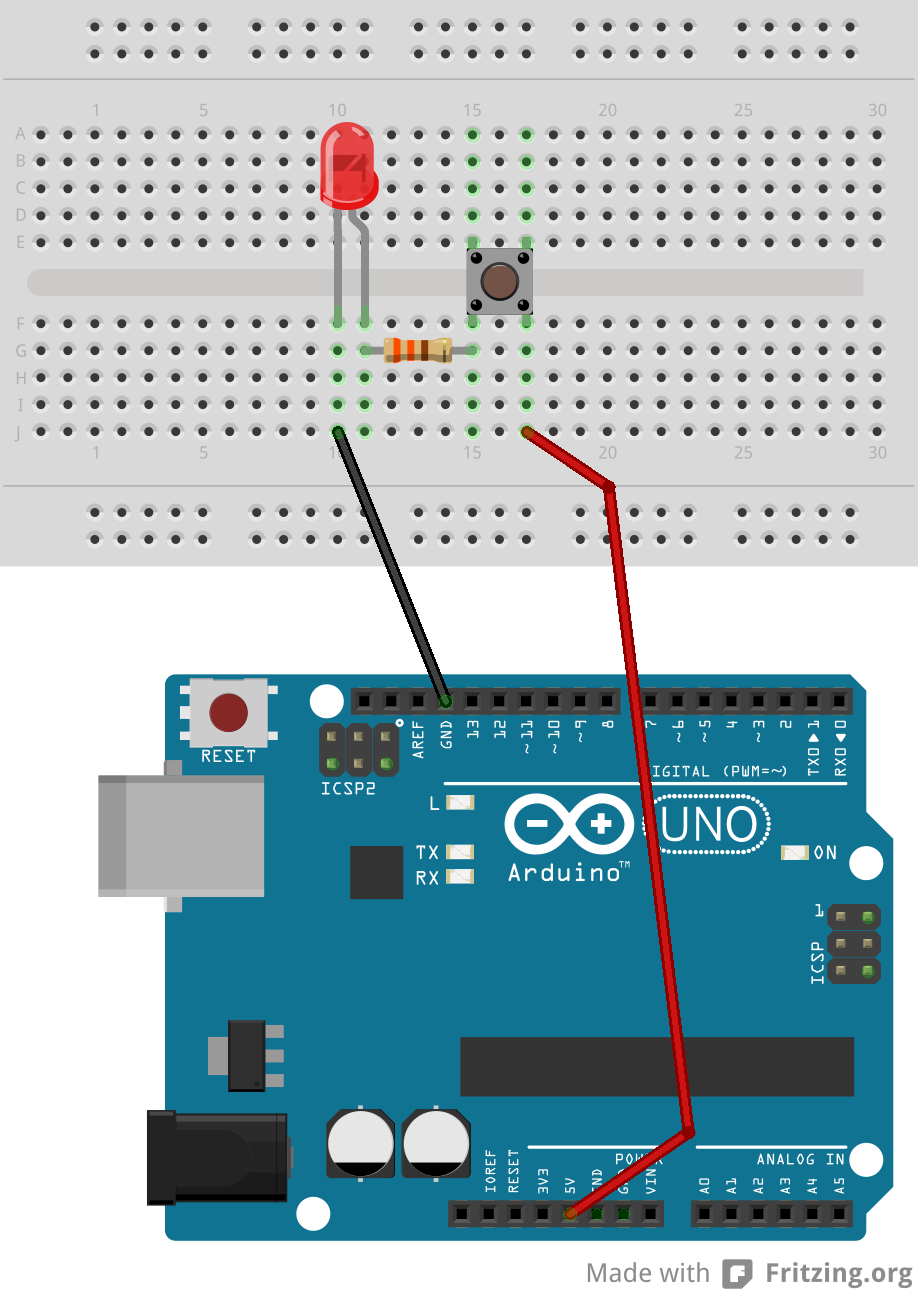
\includegraphics[width=6cm]{img/05_pushbutton_01_bb} \ \ 
  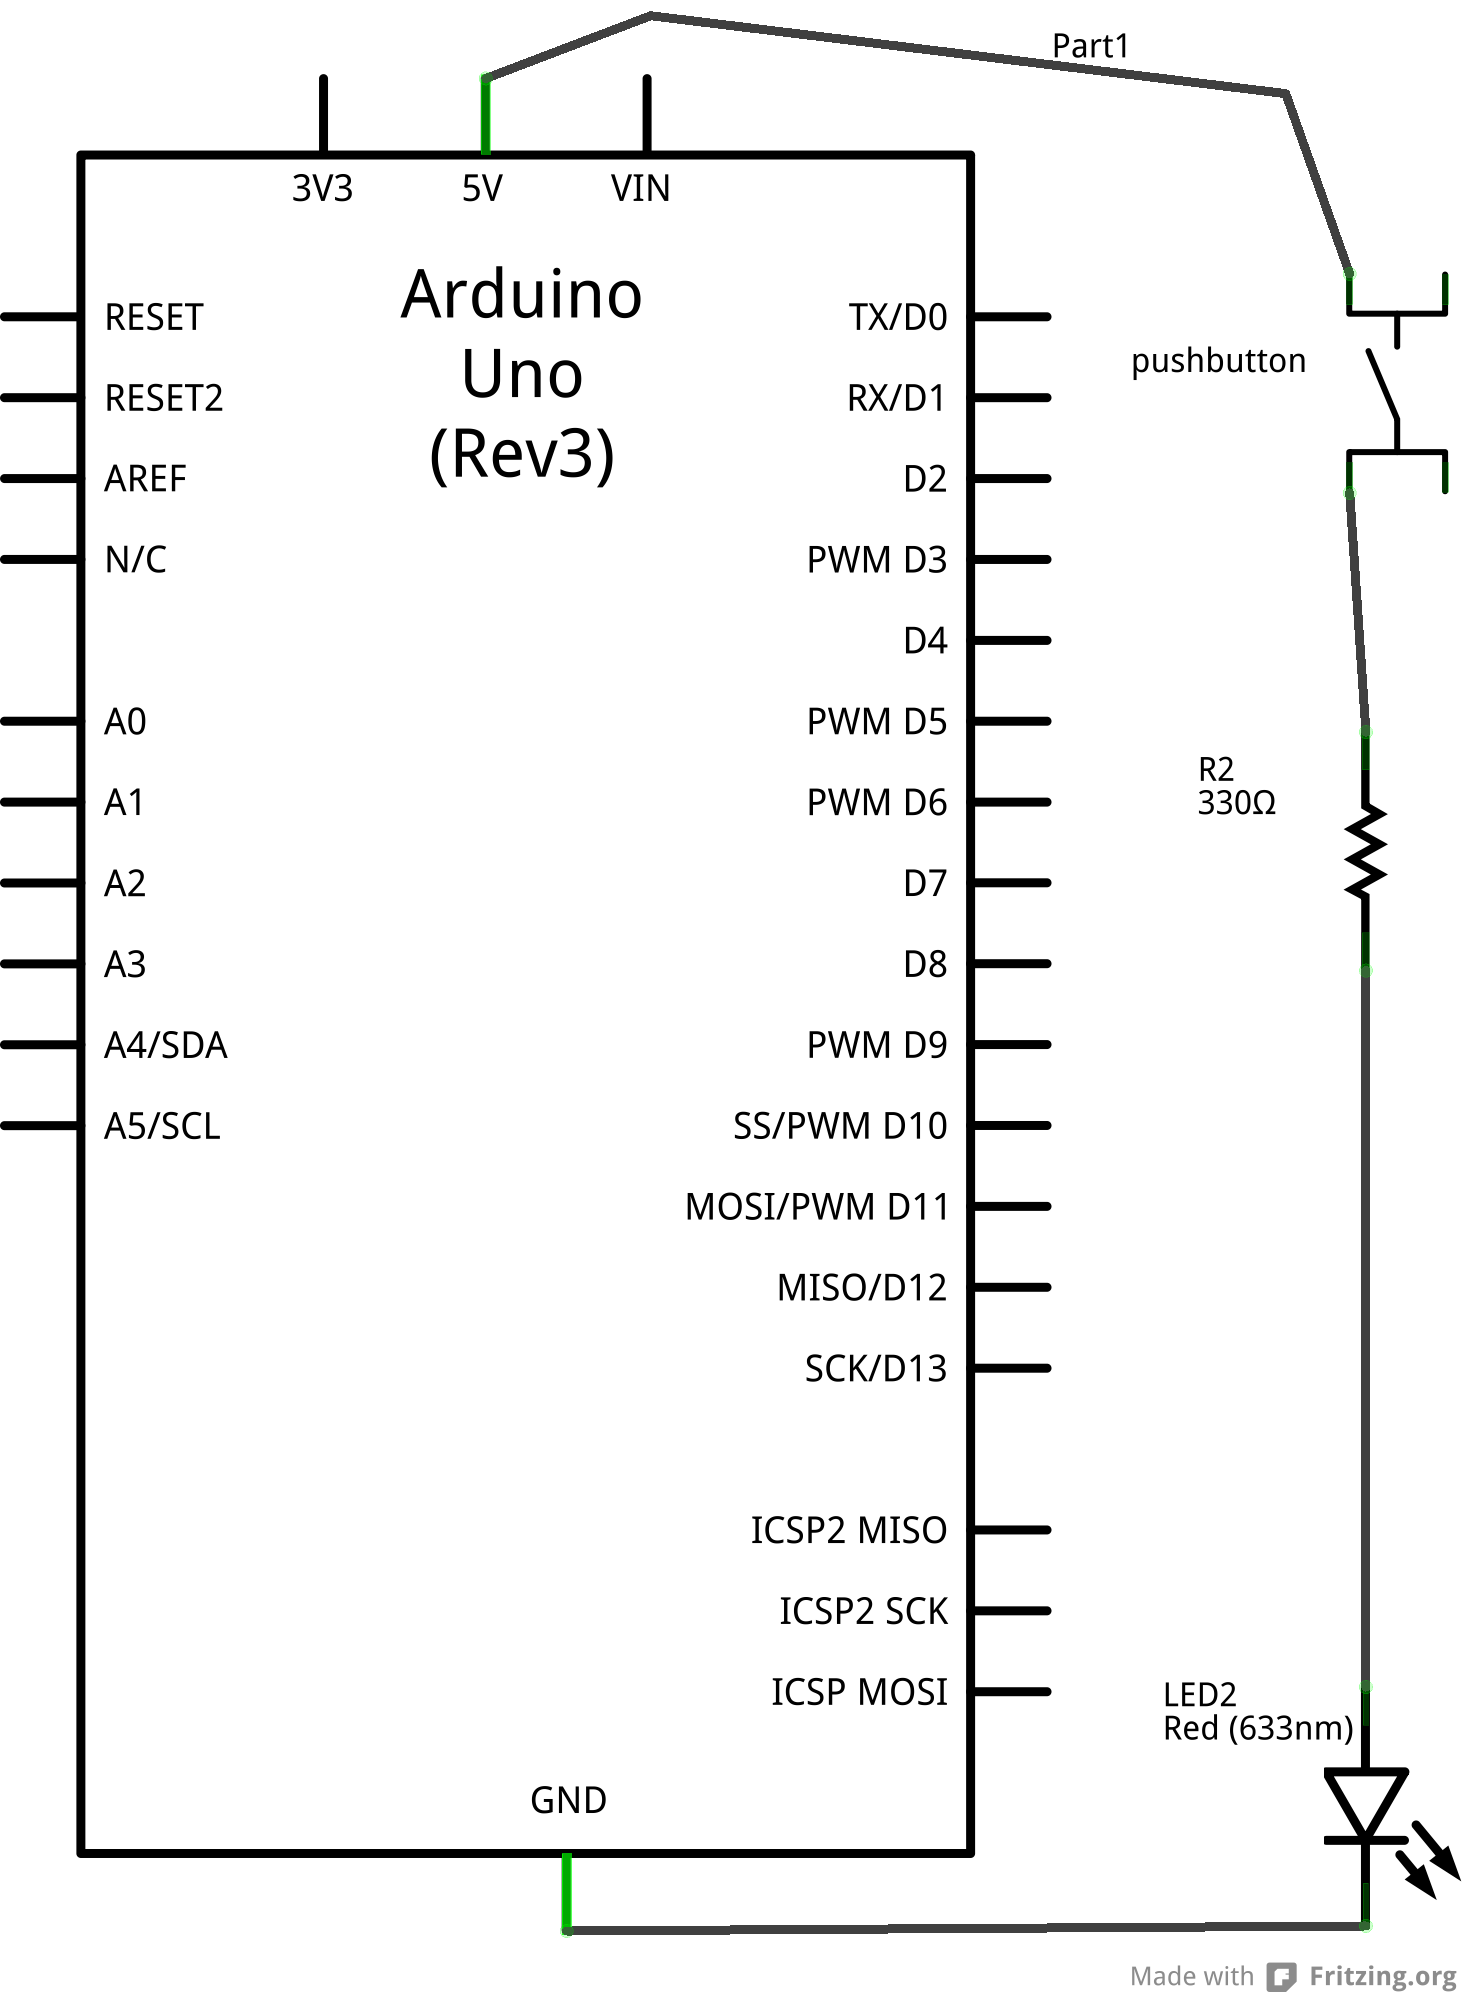
\includegraphics[width=6cm]{img/05_pushbutton_01_schem}
\caption{\engt{Power, a pushbutton and a LED, and you can control the LED. No Arduino code needed!}
\nedt{Stroom, een drukknop en een LED, en je can de LED sturen. Geen Arduino code nodig!}}
\label{f:lesson5_pbtn1}       % Give a unique label
\end{figure}

\subsection{\engt{Reading pushbutton state} \nedt{Drukknop status lezen}}

\eng{In the previous exercise we have learnt that we can use a push button to interrupt the current. That can be useful in some circumstances, but not for our Fe Cube. Instead, we want to use the button to receive input from the user. In other words, we want to know if the user pressed the button or not, and then react to that with Arduino code.

The Arduino has a special function to read input from a digital pin: \ardo{digitalRead(pin)}. To use this method, a pin must be defined as \ardo{INPUT} in the \ardo{setup} function: \ardo{pinMode(pin, INPUT);}. 

The function will read \ardo{HIGH} if the pin is on 5V, and \ardo{LOW} when on GND. So the trick is to create a circuit that is \ardo{LOW} when the button is not pressed, and \ardo{HIGH} when the button is pressed. Such a circuit is given in Figure \ref{f:lesson5_pbtn2}.
}
\ned{In de vorige oefening hebben we geleerd dat een drukknop de stroom kan onderbreken. Dit kan nuttig zijn in sommige omstandigheden, maar niet voor onze Fe Kubus. In de plaats willen we een knop waardoor we input kunnen krijgen van de gebruiker. In andere woorden, we willen weten als de gebruiker de knop drukt of niet, en we willen daarop reageren via Arduino code.

De Arduino heeft een speciale functie om input te lezen van een digitale pin:\ardo{digitalRead(pin)}. Om deze methode te gebruiken moeten we een pin defini\"eren als \ardo{INPUT} in de \ardo{setup} function: \ardo{pinMode(pin, INPUT);}. 

De functie zal \ardo{HIGH} lezen als de pin op 5V staat en \ardo{LOW} als ze op GND is. De truck is dus om een circuit te maken die  \ardo{LOW} is als de knop niet ingedrukt is en \ardo{HIGH} als de knop ingedrukt is. Zo'n circuit is gegeven in Figuur \ref{f:lesson5_pbtn2}.
}

\begin{figure}
  \centering
  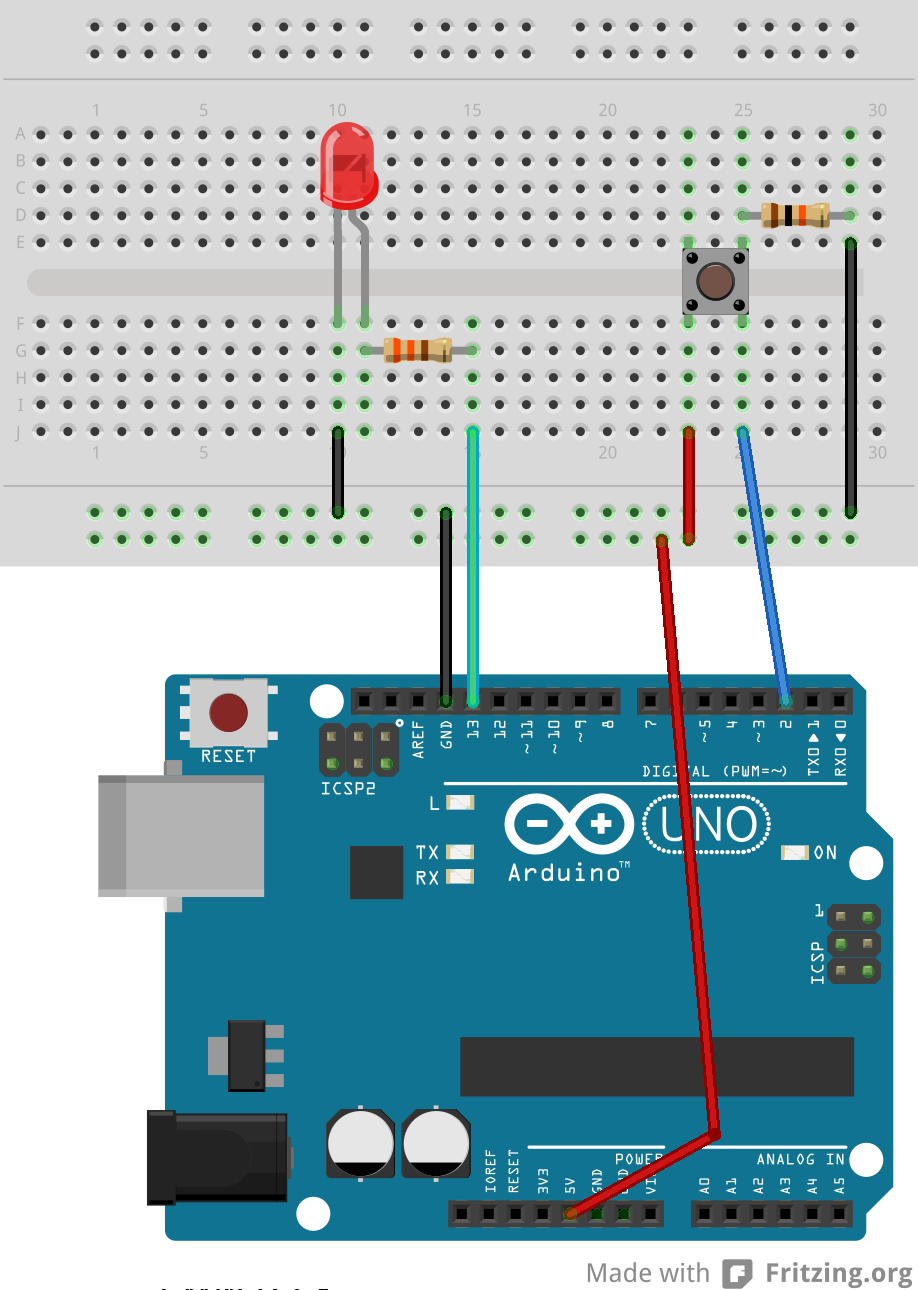
\includegraphics[width=6cm]{img/05_pushbutton_02_bb} \ \ 
  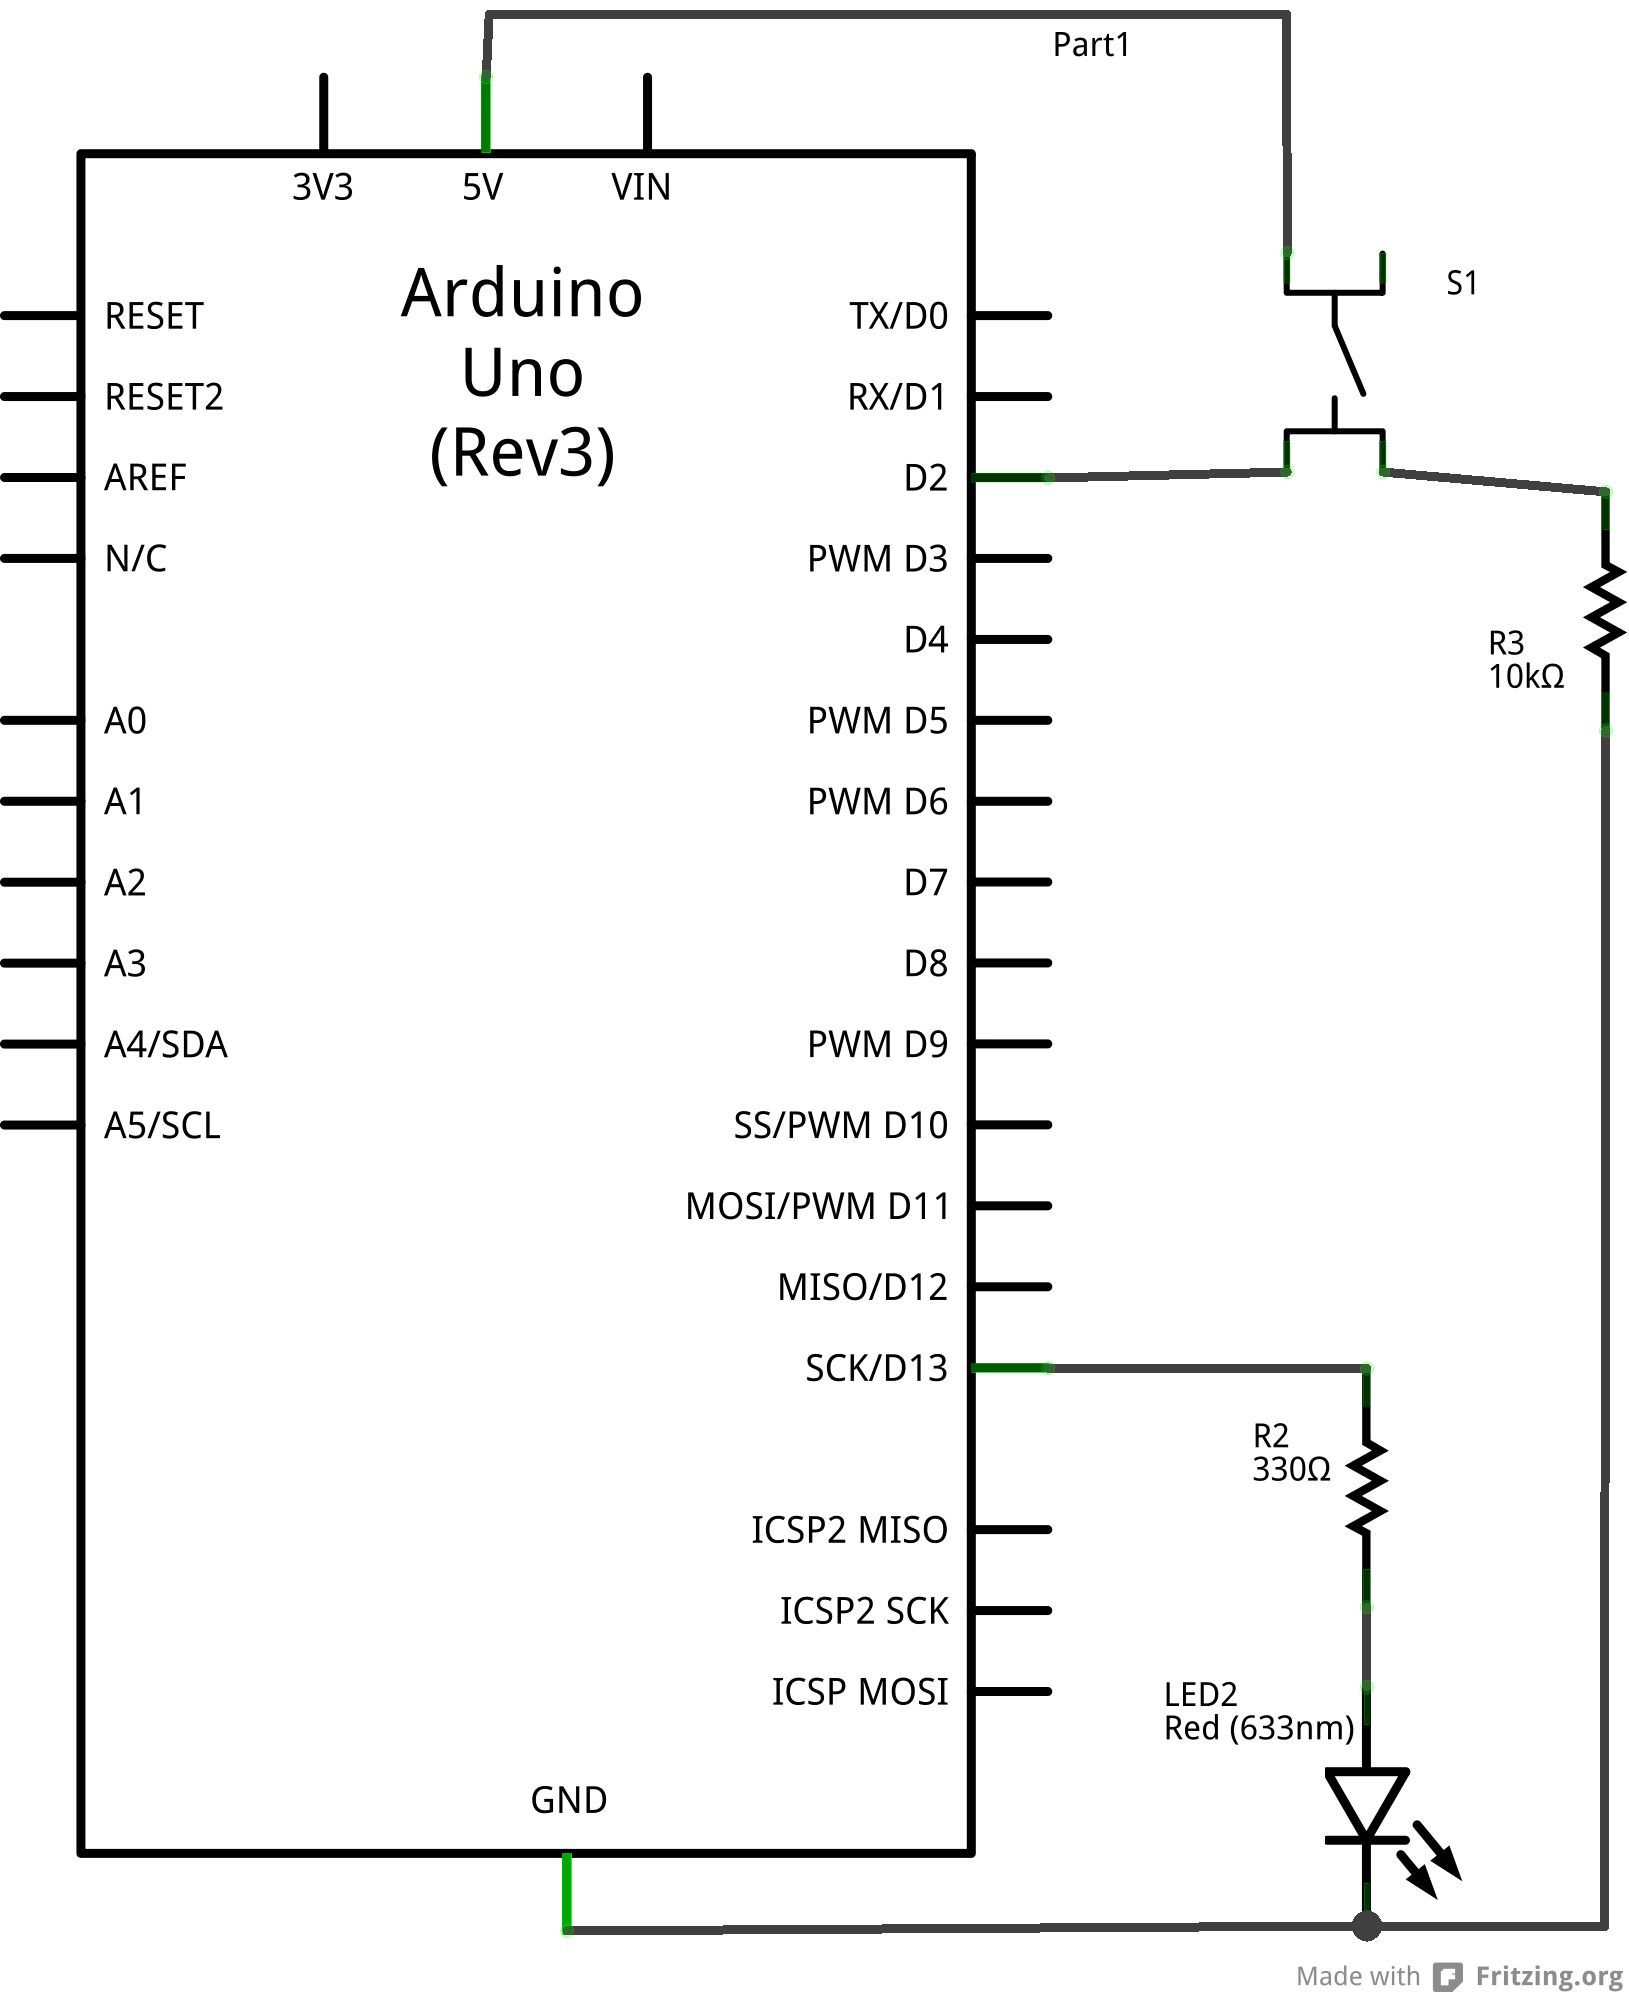
\includegraphics[width=6cm]{img/05_pushbutton_02_schem}
\caption{\engt{Reading the state of a pushbutton to control a LEDs state.}
\nedt{De status van een drukknop lezen om de staat van een LED te beheren.}}
\label{f:lesson5_pbtn2}       % Give a unique label
\end{figure}

\eng{Let's analyse this circuit. The pin to read the state of the button is pin 2. When the button is not pressed we see that the pin is connected via black to the GND. So it will be in state GND or \ardo{LOW}. You can see there is a resistor, but this seems to have no function.

Now consider the button pressed. There is a connection now from left to right in the pushbutton. So black (GND) is connected to red which goes so 5V on the Arduino. If there would be no resistor we would have a short-circuit: current running freely from 5V to GND. So, we \textbf{need} a resistor to avoid a short-circuit! What resistor do we need? Well, we want to have at pin 2, 5V when the button is pushed down, \textbf{and} we don't want to spend a lot of current to achieve this state. Hence, we want a large resistor! A large resistor will make sure the resistance from the wires from the pushbutton to the 5V pin is neglectable compared to the large resistor, so pin 2 will be on 5V. At the same time, a large resistor will make sure very little current will actually flow over the pushbutton, so our circuit will be very efficient. So, take for this resistor 10000$\Omega$ which we write as 10K$\Omega$ or 10k$\Omega$. We call such a resistor used in this way a pull-down or pull-up resistor.

We can now write Arduino code that reads the state of pin 2, and let's the LED shine based on this. To achieve this, our LED circuit of the previous excercise must be changed to draw current from a pin, eg pin 13. Like that, setting pin 13 HIGH or LOW will control the LED. Note that most Arduino boards have a tiny LED connected to pin 13 on the board, so you could use that instead of a real LED. The code is given in Code
\ref{c:pbtn}.

Note that our circuit works exactly as the one in the previous excercise: the LED shines when the button is pressed. How we achieve this is completely different though.
}
\ned{Laat ons dit circuit analyseren. De pin om de status van de knop te lezen is pin 2. Als deze knop niet is ingedrukt zien we dat de pin verbonden is via zwart met de GND. Het zal dus in de GND staat of \ardo{LOW} zijn. Je ziet dat er een weerstand is, maar deze lijkt geen functie te hebben.

Beschouw nu het geval dat de knop ingedrukt is. Er is nu een connectie van links naar rechts in de drukknop. Zwart (GND) is dus verbonden met rood die naar de 5V op de Arduino gaat. Moest er geen weerstand zijn dan zouden we een kortsluiting krijgen: stroom die vrij stroomt van 5V naar GND. Aldus \textbf{moeten} we een weerstand hebben om kortsluiting te voorkomen. Welke weerstand hebben we nodig? Wel, we willen dat pin 2 op 5V staat als de knop ingedrukt is, \textbf{\'en} we willen niet veel stroom gebruiken om dit te verkrijgen. Bijgevolg willen we een grote weerstand! 
Een grote weerstand zal zorgen dat de weerstand in de draden van de drukknop naar de 5V pin verwaarloosbaar is ten opzichte van de grote weerstand, en dus zal pin 2 op 5V staan. Terzelfdertijd zal een grote weerstand ervoor zorgen dat er maar heel weinig stroom zal vloeien over de drukknop, en ons circuit zal dus heel efficient zijn. Neem daarom als weerstand eentje van 10000$\Omega$, welke we ook schrijven als 10K$\Omega$ of 10k$\Omega$. We noemen zo'n weerstand op deze manier gebruikt een \textit{pull-down} (naar GND) of \textit{pull-up} (naar 5V) weerstand.

We kunnen nu Arduino code schrijven die de status van pin 2 leest, en de LED laten schijnen op basis van die status. Om dit te doen dient ons LED circuit van de vorige oefening aangepast te worden om stroom te trekken van een pin, bv pin 13. Zo kunnen we pin 13 HIGH of LOW zetten om de LED te beheren. Merk op dat de meeste Arduino borden een kleine LED op het bord hebben die verbonden is met pin 13, je zou dus dat kunnen gebruiken ipv een echte LED. De code is gegeven in Code \ref{c:pbtn}. 
}

\begin{code}\label{c:pbtn}
 \ \newline
\inputardfull{\string"../sketches/Fe_cube_05_pbtn/Fe_cube_05_pbtn.ino\string"}
\end{code}

\subsection{\engt{Only one button?} \nedt{Maar \'e\'en knop?}}

\eng{What can we do with only one button? More than you think! Consider a touch pad on a tablet. What can you do with one finger? Consider a mouse. What can you do with one button?

Yes, the answer is: a lot! You can have a normal press, a long press, a double press. And you could even react differently to input in certain patterns (gestures). 
Reacting differently to different presses is a matter of software. The better you program, the better you can react to things happening. So, we need to think a bit on a method to program reacting to different presses.

Let's define some concepts:
\begin{itemize}
 \item \textbf{Input sampling}. We don't want to spend too much time observing what happens to the button. Testing the state of the button every 40 ms (the time of a frame in our Fe Cube) should be sufficient. It might be a good idea to not block the normal code running on our Arduino, so to let that code indicate when we are allowed to sample the input, in our case the button.
 \item An \textbf{event} is something happening to the button. There are only two events: \textit{buttonpress} and \textit{buttonrelease}. As we have seen from the previous excercise, we can recognize these events by a change in state. The first is LOW to HIGH, and the second is HIGH to LOW
 \item Next we have \textbf{event handling}. Event handling is converting events in a \textit{button press type}. To do event handling, we need to know the time since a previous event, as well as the type of a previous press type. We can distinguish like this:
\begin{enumerate}
 \item \textbf{short press}: a press and a release within 2 seconds
 \item \textbf{long press}: a press and a release taking more than 2 seconds
 \item \textbf{double press}: a short press within 0.5 seconds after a previous short press
 \item \textbf{extreme long press}: a press longer than 4 seconds. No need to wait for the release to set a press type.
\end{enumerate}
 \item An \textit{INTERRUPT}. We will have code running on our Arduino, and a button being pressed. We need to be able to interrupt the code that runs to start something else. So, our code will observe the button press type and based on that interrupt the running code to react to the press.
\end{itemize}
}

\ned{Wat kunnen we doen met maar \'e\'en knop? Meer dan je denkt! Denk aan een aanraakscherm op een tablet. Wat kun je doen met \'e\'en vinger? Denk aan de computermuis. Wat kun je doen met \'e\'en knop?

Ja, het antwoord is: veel! Je kan een normale druk hebben, een lange druk, een dubbele druk ... . Je zou zelf kunnen reageren op basis van bepaalde patronen (bv SOS in morse).
Het verschillend reageren op verschillende drukken is een kwestie van software. Hoe beter je programmeert hoe beter je kan reageren op dingen die gebeuren. We moeten dus een beetje nadenken over de methode om met een programma te reageren op een knop.

Laat ons enkele concepten defini\"eren:
\begin{itemize}
 \item \textbf{Input sampling} of \textbf{Invoertesten}. We willen niet teveel tijd besteden met het observeren wat er gebeurt met de knop. De status van de knop elke 40 ms testen (de tijd van een frame in onze Fe Cubus) zou voldoende moeten zijn. Het is misschien een goed idee om de gewone code die loopt op de Arduino niet te blokkeren, en we zouden dus die code kunnen laten aangeven wanneer we de invoer mogen testen, in ons geval de knop.
 \item Een \textbf{event} of \textbf{gebeurtenis} is iets dat gebeurt met de knop. Er zijn maar twee mogelijke events : \textit{buttonpress} and \textit{buttonrelease}, in het Nederlands: Knop indrukken en Knop loslaten. Zoals we in de vorige oefening gezien hebben kunnen we deze herkennen door een verandering in de status van de knop. De eerste is LOW naar HIGH en de tweede HIGH naar LOW.
 \item Vervolgens hebben we \textbf{event handling}. Event handling is het omzetten van events naar \textit{button press type}. Om event handling te doen moeten we de tijd weten sinds een vorig event alsook het type van de vorige druk. Op deze manier kunnen we onderscheiden:
\begin{enumerate}
 \item \textbf{short press} of \textbf{korte druk}: een druk en loslaten binnen de 2 seconden
 \item \textbf{long press} of \textbf{lange druk}: een druk en loslaten die langer dan 2 seconden duurt
 \item \textbf{double press} of \textbf{dubbele druk}: a korte druk binnen de 0.5 seconden na een vorige korte druk
 \item \textbf{extreme long press} of \textbf{extreem lange druk}: een druk die langer dan 4 seconden duurt. Het is dan niet nodig te wachten op een loslaten om het druk type vast te leggen.
\end{enumerate}
 \item Een \textit{INTERRUPT}. Dit is het Engels voor \textit{Onderbreking}. We zullen code hebben lopen op de Arduino, en een knop die gedrukt wordt. We dienen in staat te zijn de code te onderbreken om iets anders te doen. Onze code moet dus het butten press type observeren en op basis daarvan de code kunnen onderbreken om te reageren op de druk.
\end{itemize}
}

\eng{
These are a lot of concepts to include in our code. Let's create code that does different things to the LED, to see how we can do this in practice, see Code \ref{c:pbtn_event}.

This code contains in the first part a function to do inputsampling, called \ardo{inputsampling()}. This happens if the variable \ardo{allowInput} allos it. The input is then handled in the function  \ardo{eventhandling}. This function first determines the \ardo{event}, and then determiens the press type, which is saved in the variable \ardo{presstype}.

The second part of the code is the program that controls our LED. We can switch the LED on or off via a long press. A short press dims the LED a small fraction. After 15 short presses the LED will be at it's minimum brightness, with the next press going back to full brightness. We use PWM to dim the light, so we use for example pin 11. A double press will be translated in a flickering LED: half a second on, then half a second off.

This code will observe the variable \ardo{presstype}, and if it is different from \ardo{NOPRESS} do the desired action. After handling the press type, we put  \ardo{presstype=NOPRESS}, so that we again wait for the next input.

You have written your first program that allows you to control how the Arduino works!
}

\ned{Dit zijn veel concepten om op te nemen in onze code. Laat ons nu code maken die verschillende dingen doet met de LED, om te zien hoe we dit in de praktijk kunnen doen, zie Code \ref{c:pbtn_event}. 

In deze code bevat het eerste gedeelte een functie die invoertesten doet, \ardo{inputsampling()} als dit toegelaten is door de variabele \ardo{allowInput}. De invoer wordt dan verwerkt met de functie \ardo{eventhandling}. Deze functie bepaalt eerst het \ardo{event}, en daarna het type druk, welke opgeslagen wordt in de variabele \ardo{presstype}. 

Het tweede deel van de code is dan ons programma die een LED doet branden. We kunnen via een lange druk de LED aan of af doen. Een korte druk dimt de LED een kleine fractie. Na 15 keer een korte druk zal de LED maximaal gedimd zijn, om daarna weer op volle sterkte te branden. We gebruiken PWM om te dimmen, dus gebruiken we bv pin 11 voor de LED. Een dubbele druk zullen we vertalen in het flikkeren van de LED: een halve seconde aan, een halve uit. 

Deze code zal dus de variabele \ardo{presstype} observeren, en als deze verschillend is van \ardo{NOPRESS} de geweste actie ondernemen. Na het behandelen van een druktype zetten we \ardo{presstype=NOPRESS}, zodat we weer wachten op de volgende input.

Je hebt je eerste programma nu af die je toelaat te sturen hoe je Arduino werkt!
}

\begin{code}\label{c:pbtn_event}
 \ \newline
\inputardfull{\string"../sketches/Fe_cube_05_pbtn_events/Fe_cube_05_pbtn_events.ino\string"}
\end{code}


\subsection{\engt{Fe Cube + pushbutton = control} \nedt{Fe Cube + Drukknop = sturing}}

\eng{We have our Fe Cube, and we have the circuit for pushbutton input. So it's only a matter of combining the two, and then adapting our Cube program to react to specific press input. The combined wiring is shown in Figure \ref{f:lesson5_pbtn3} for the breadboard setup. Integrate it in your Fe Cube.
}

\ned{We hebben onze Fe Kubus, en we hebben een circuit om de drukknop te gebruiken. Het is dus enkel een kwestie van beiden te combineren, en om dan ons Kubus programma aan te passen om te reageren op specifieke druk input. De gezamelijke bekabeling is te zien in  Figuur \ref{f:lesson5_pbtn3} voor het schakelbord. Integreer ze in je Fe Kubus.
}

\begin{figure}
  \centering
  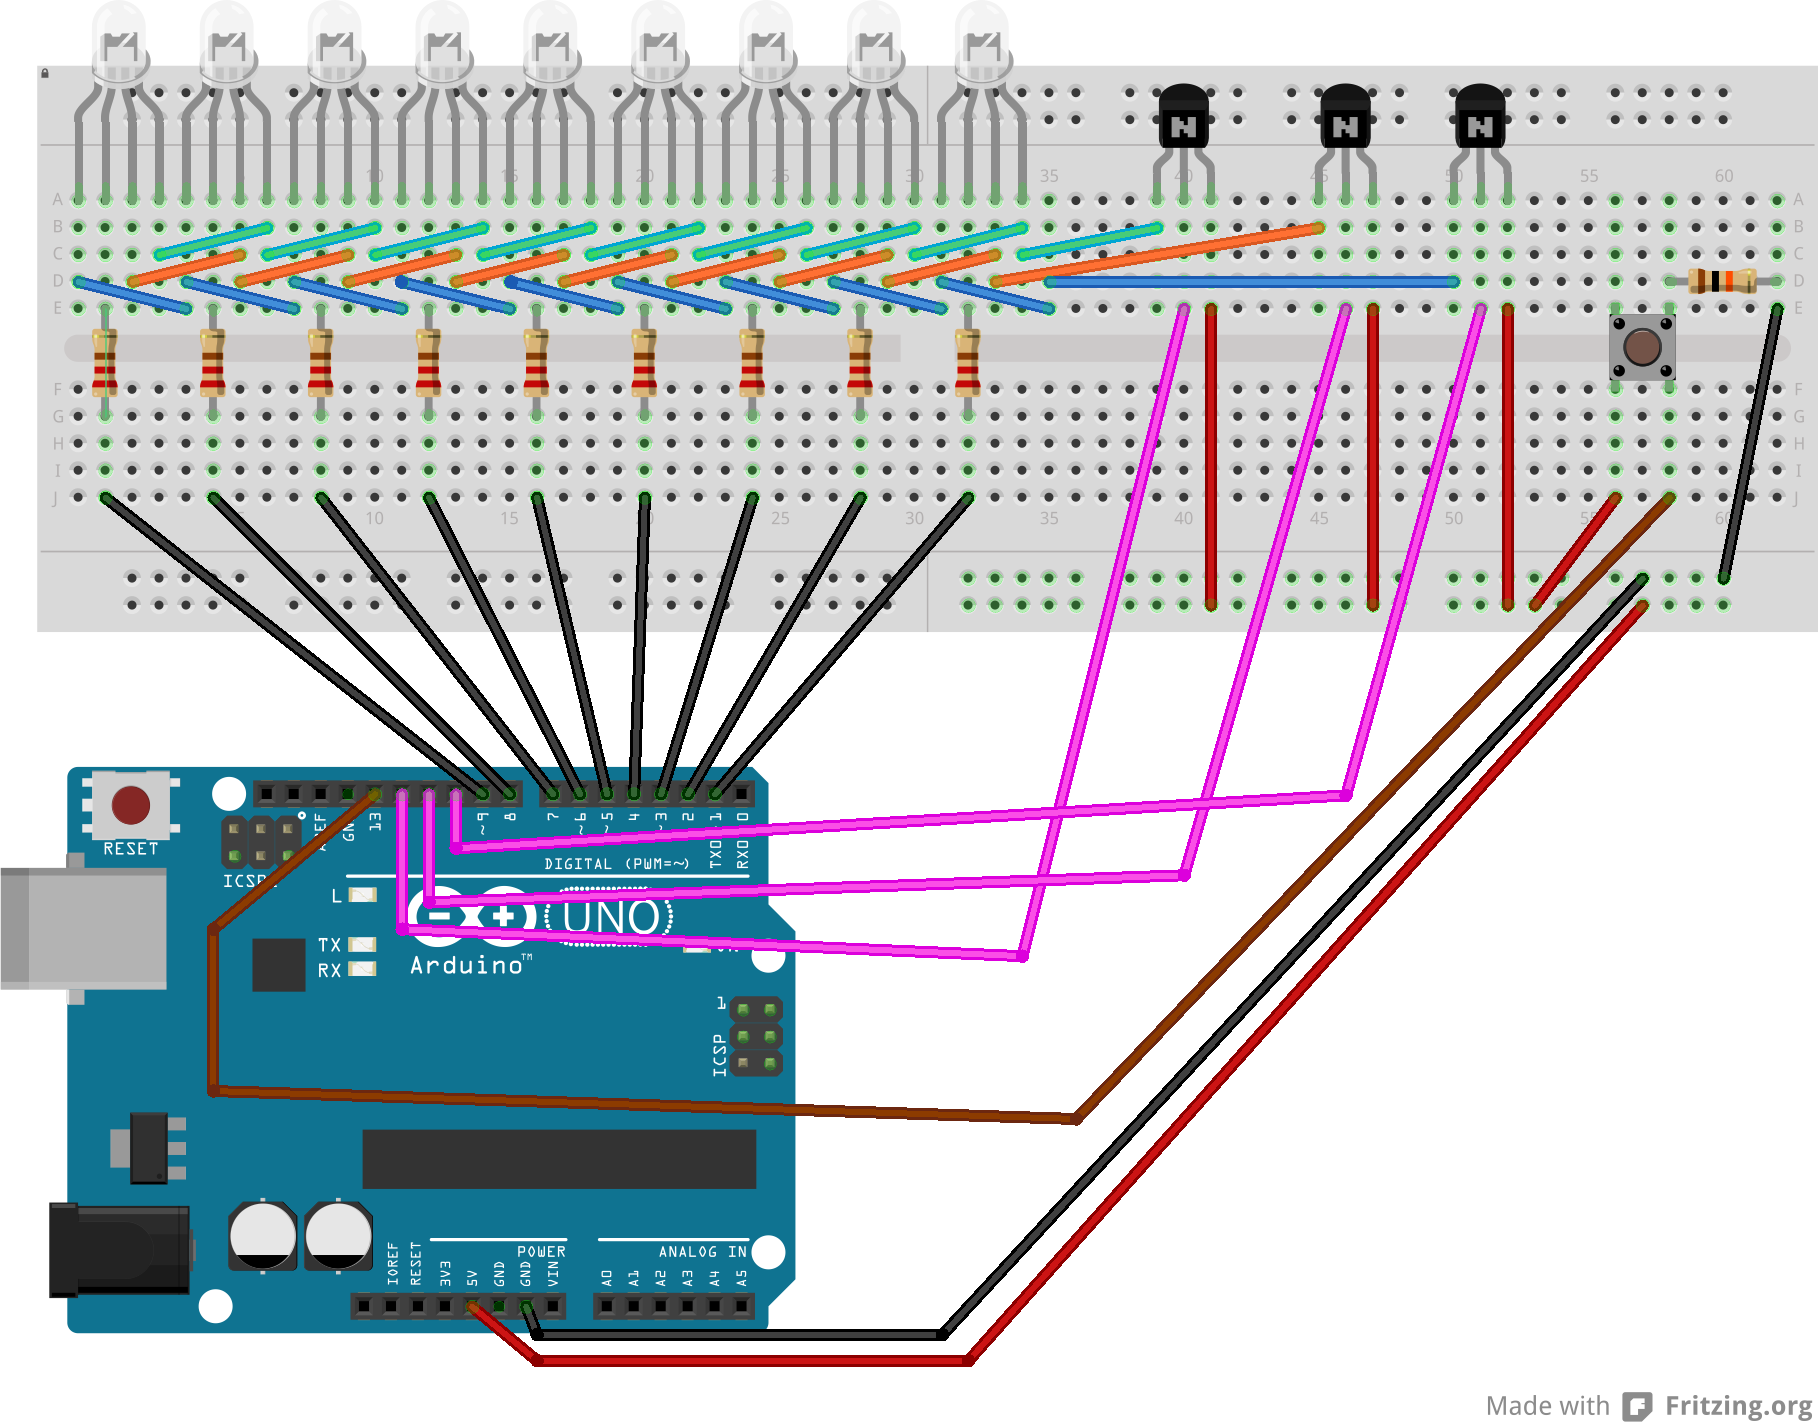
\includegraphics[width=6cm]{img/05_pushbutton_03_cube_bb} \ \ 
  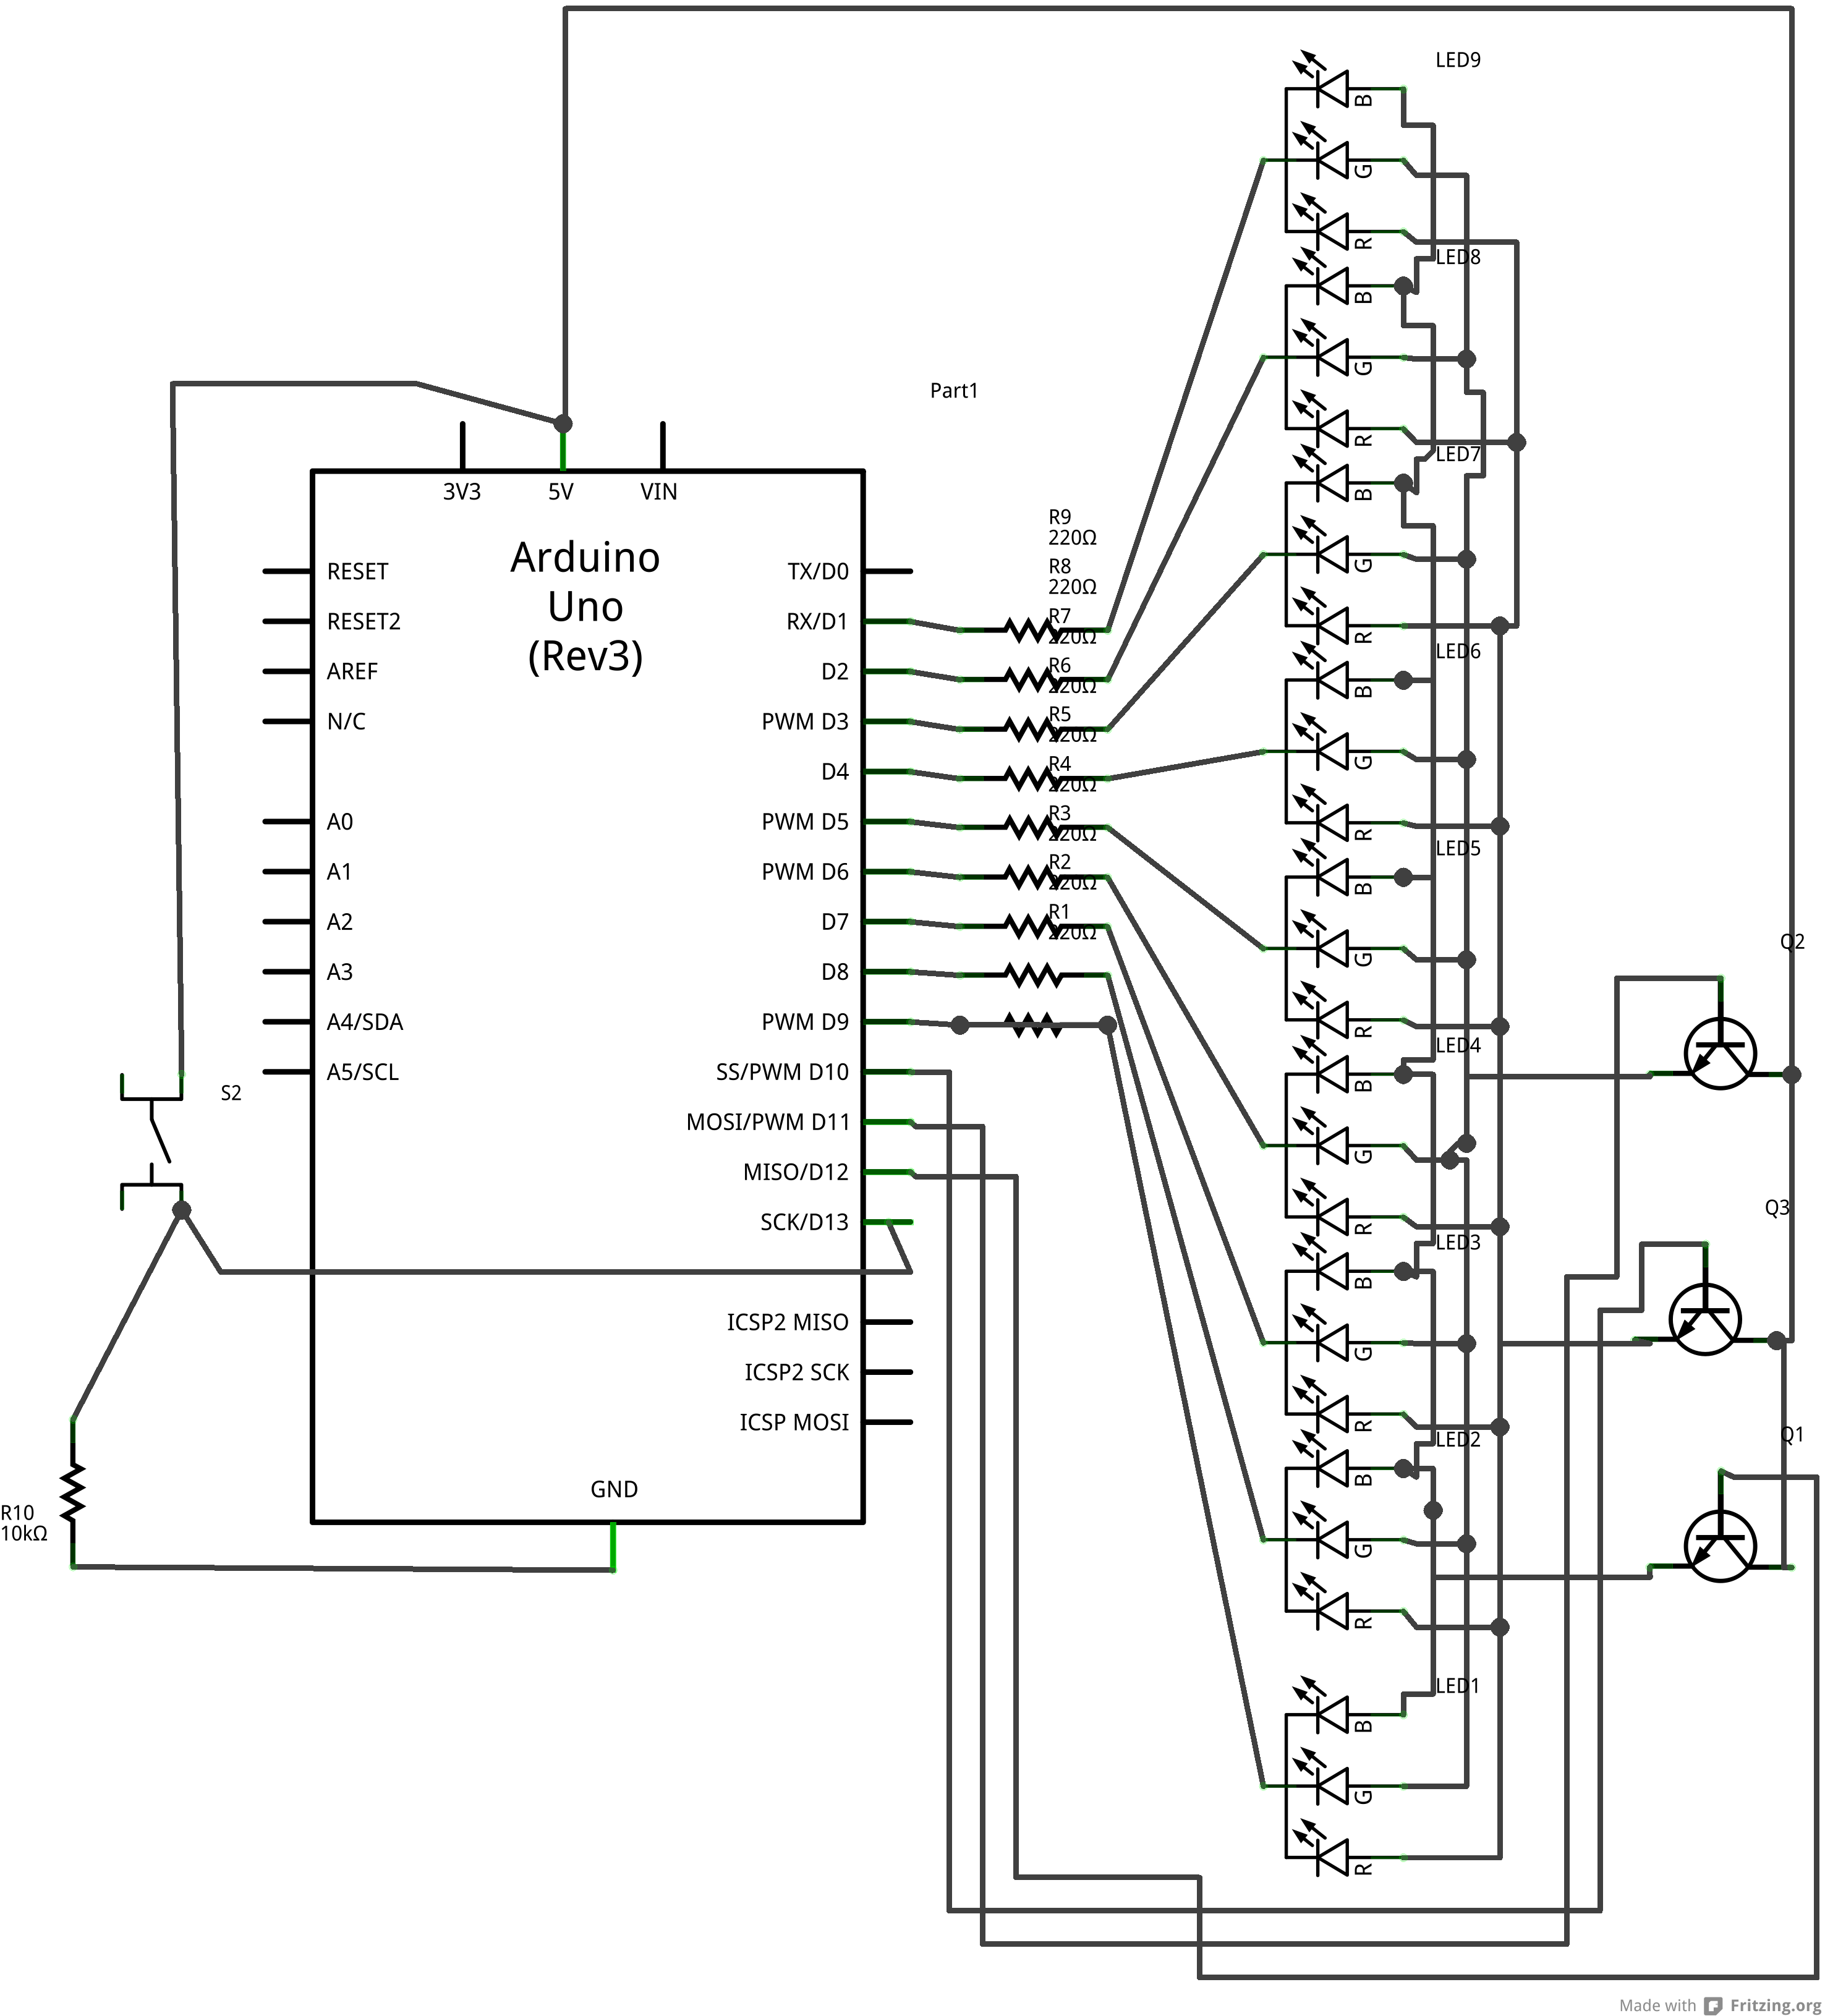
\includegraphics[width=6cm]{img/05_pushbutton_03_cube_schem}
\caption{\engt{The same pushbutton wiring can be used with the Fe Cube as we still have
a digital pin free}
\nedt{Dezelfde drukknop bekabeling kan gebruikt worden met de Fe Kubus gezien we nog een vrije digitale pin hebben}}
\label{f:lesson5_pbtn3}
\end{figure}

\eng{For the code, we need to combine our Cube code, with the pushbutton code. The entire button handling code can be copied verbatim. In the Cube code we need to do the following changes:
\begin{itemize}
 \item We no longer update the \ardo{NRPATTERN} variable when a pattern is finished. The user will need to press the button to change the pattern.
 \item In the \ardo{loop()} function we start with the inputsampling. Next the presstype is checked. If the button press type is \ardo{NOPRESS} and the shot is not finished, no new shot will be started. In all other cases we handle the press type. We will do the following: if a shortpress, we increase \ardo{NRPATTERN}, so as to move to the next pattern. If \ardo{EXTREMEPRESS} we will switch the cube off or on. If \ardo{DOUBLEPRESS} we will show a new effect: rolling 3 dices.
 \item We write new shots: one to switch off the cube, and one for dice rolling
 \item We update the \ardo{movie} function: if we need to show the dice effect or switch off the LED, we return those shots. Otherwise we do as before: return the correct pattern.
\end{itemize}
The full code is in \url{https://github.com/ingegno/fecube/blob/master/sketches/Fe_cube_05_cube_pbtn/Fe_cube_05_cube_pbtn.ino}.
}

\ned{In de code dienen we de kubus code te combineren met de drukknop code. De volledige drukknop logica kan letterlijk overgenomen worden. In de oorspronkelijke kubus code moeten we wel nog volgende wijzigingen doen:
\begin{itemize}
 \item We passen de variabele \ardo{NRPATTERN} niet langer aan als het patroon af is. De gebruiker zal moeten de knop drukken om een ander effect te zien.
 \item In de \ardo{loop()} functie beginnen we met invoerlezing via de \ardo{inputsampling} functie. Vervolgens controleren we het presstype. Als de drukknop type \ardo{NOPRESS} is en het shot niet gedaan, zal er geen nieuw shot started. In alle andere gevallen moeten we het drukknop type behandelen. We zullen het volgende doen: bij een korte druk zullen we \ardo{NRPATTERN} verhogen, opdat een nieuw patroon zou getoond worden.  Indien het type \ardo{EXTREMEPRESS} is zullen we de kubus af- of aanzetten. Bij \ardo{DOUBLEPRESS} zullen we een nieuw effect tonen: 3 dobbelstenen gooien.
 \item We schrijven nieuwe shots: een om te kubus af te zetten, en een om de dobbelsteen te tonen
 \item We passen de \ardo{movie} functie aan: Als we de dobbelsteen moeten tonen of de LED moeten uitzetten, geven we die shots terug. Anders doen we zoals vroeger: het juiste patroon teruggeven.
\end{itemize}
De volledige code kun je vinden op 
\url{https://github.com/ingegno/fecube/blob/master/sketches/Fe_cube_05_cube_pbtn/Fe_cube_05_cube_pbtn.ino}.
}

